\documentclass[11pt]{article}

% Encoding and font setup
\usepackage[T1]{fontenc}
\usepackage[utf8]{inputenc}
\usepackage{lmodern}

% Page layout and micro-typography
\usepackage[margin=1in]{geometry}
\usepackage{microtype}
\usepackage{csquotes}
\usepackage{float} % for [H] exact placement of figures
\usepackage[section]{placeins} % prevent floats from crossing section boundaries
\usepackage[skip=0pt]{caption} % control caption spacing

% Math and figures
\usepackage{amsmath, amssymb}
\usepackage{graphicx}
\graphicspath{{../images/}} % look for images in the images/ folder one level up

% Remove vertical whitespace around figures
\setlength{\intextsep}{0pt}
\setlength{\textfloatsep}{0pt}
\setlength{\floatsep}{0pt}
\setlength{\dbltextfloatsep}{0pt}
\setlength{\dblfloatsep}{0pt}
\setlength{\abovecaptionskip}{0pt}
\setlength{\belowcaptionskip}{0pt}
\captionsetup[figure]{aboveskip=0pt, belowskip=0pt}

% Links
\usepackage{hyperref}
\hypersetup{colorlinks=true, linkcolor=blue, urlcolor=blue, citecolor=blue}

% Title information
\title{Project Type Synthesis Homework}
\author{Your Name}
\date{\today}

\begin{document}

\maketitle

\begin{abstract}
Briefly summarize the purpose and key findings of this document.
\end{abstract}

\tableofcontents
\newpage

\section{US4509509A: Apparatus for Treating the Joints of the Human Body}
\subsection{Description}
Early CPM concept emphasizing adjustable thigh and calf supports driven by a motorized linkage to provide controlled flexion/extension. Focuses on modular supports and variable range/speed settings to accommodate different patient anatomies and therapy progressions.
\subsection{Images}
\begin{figure}[H]
  \centering
  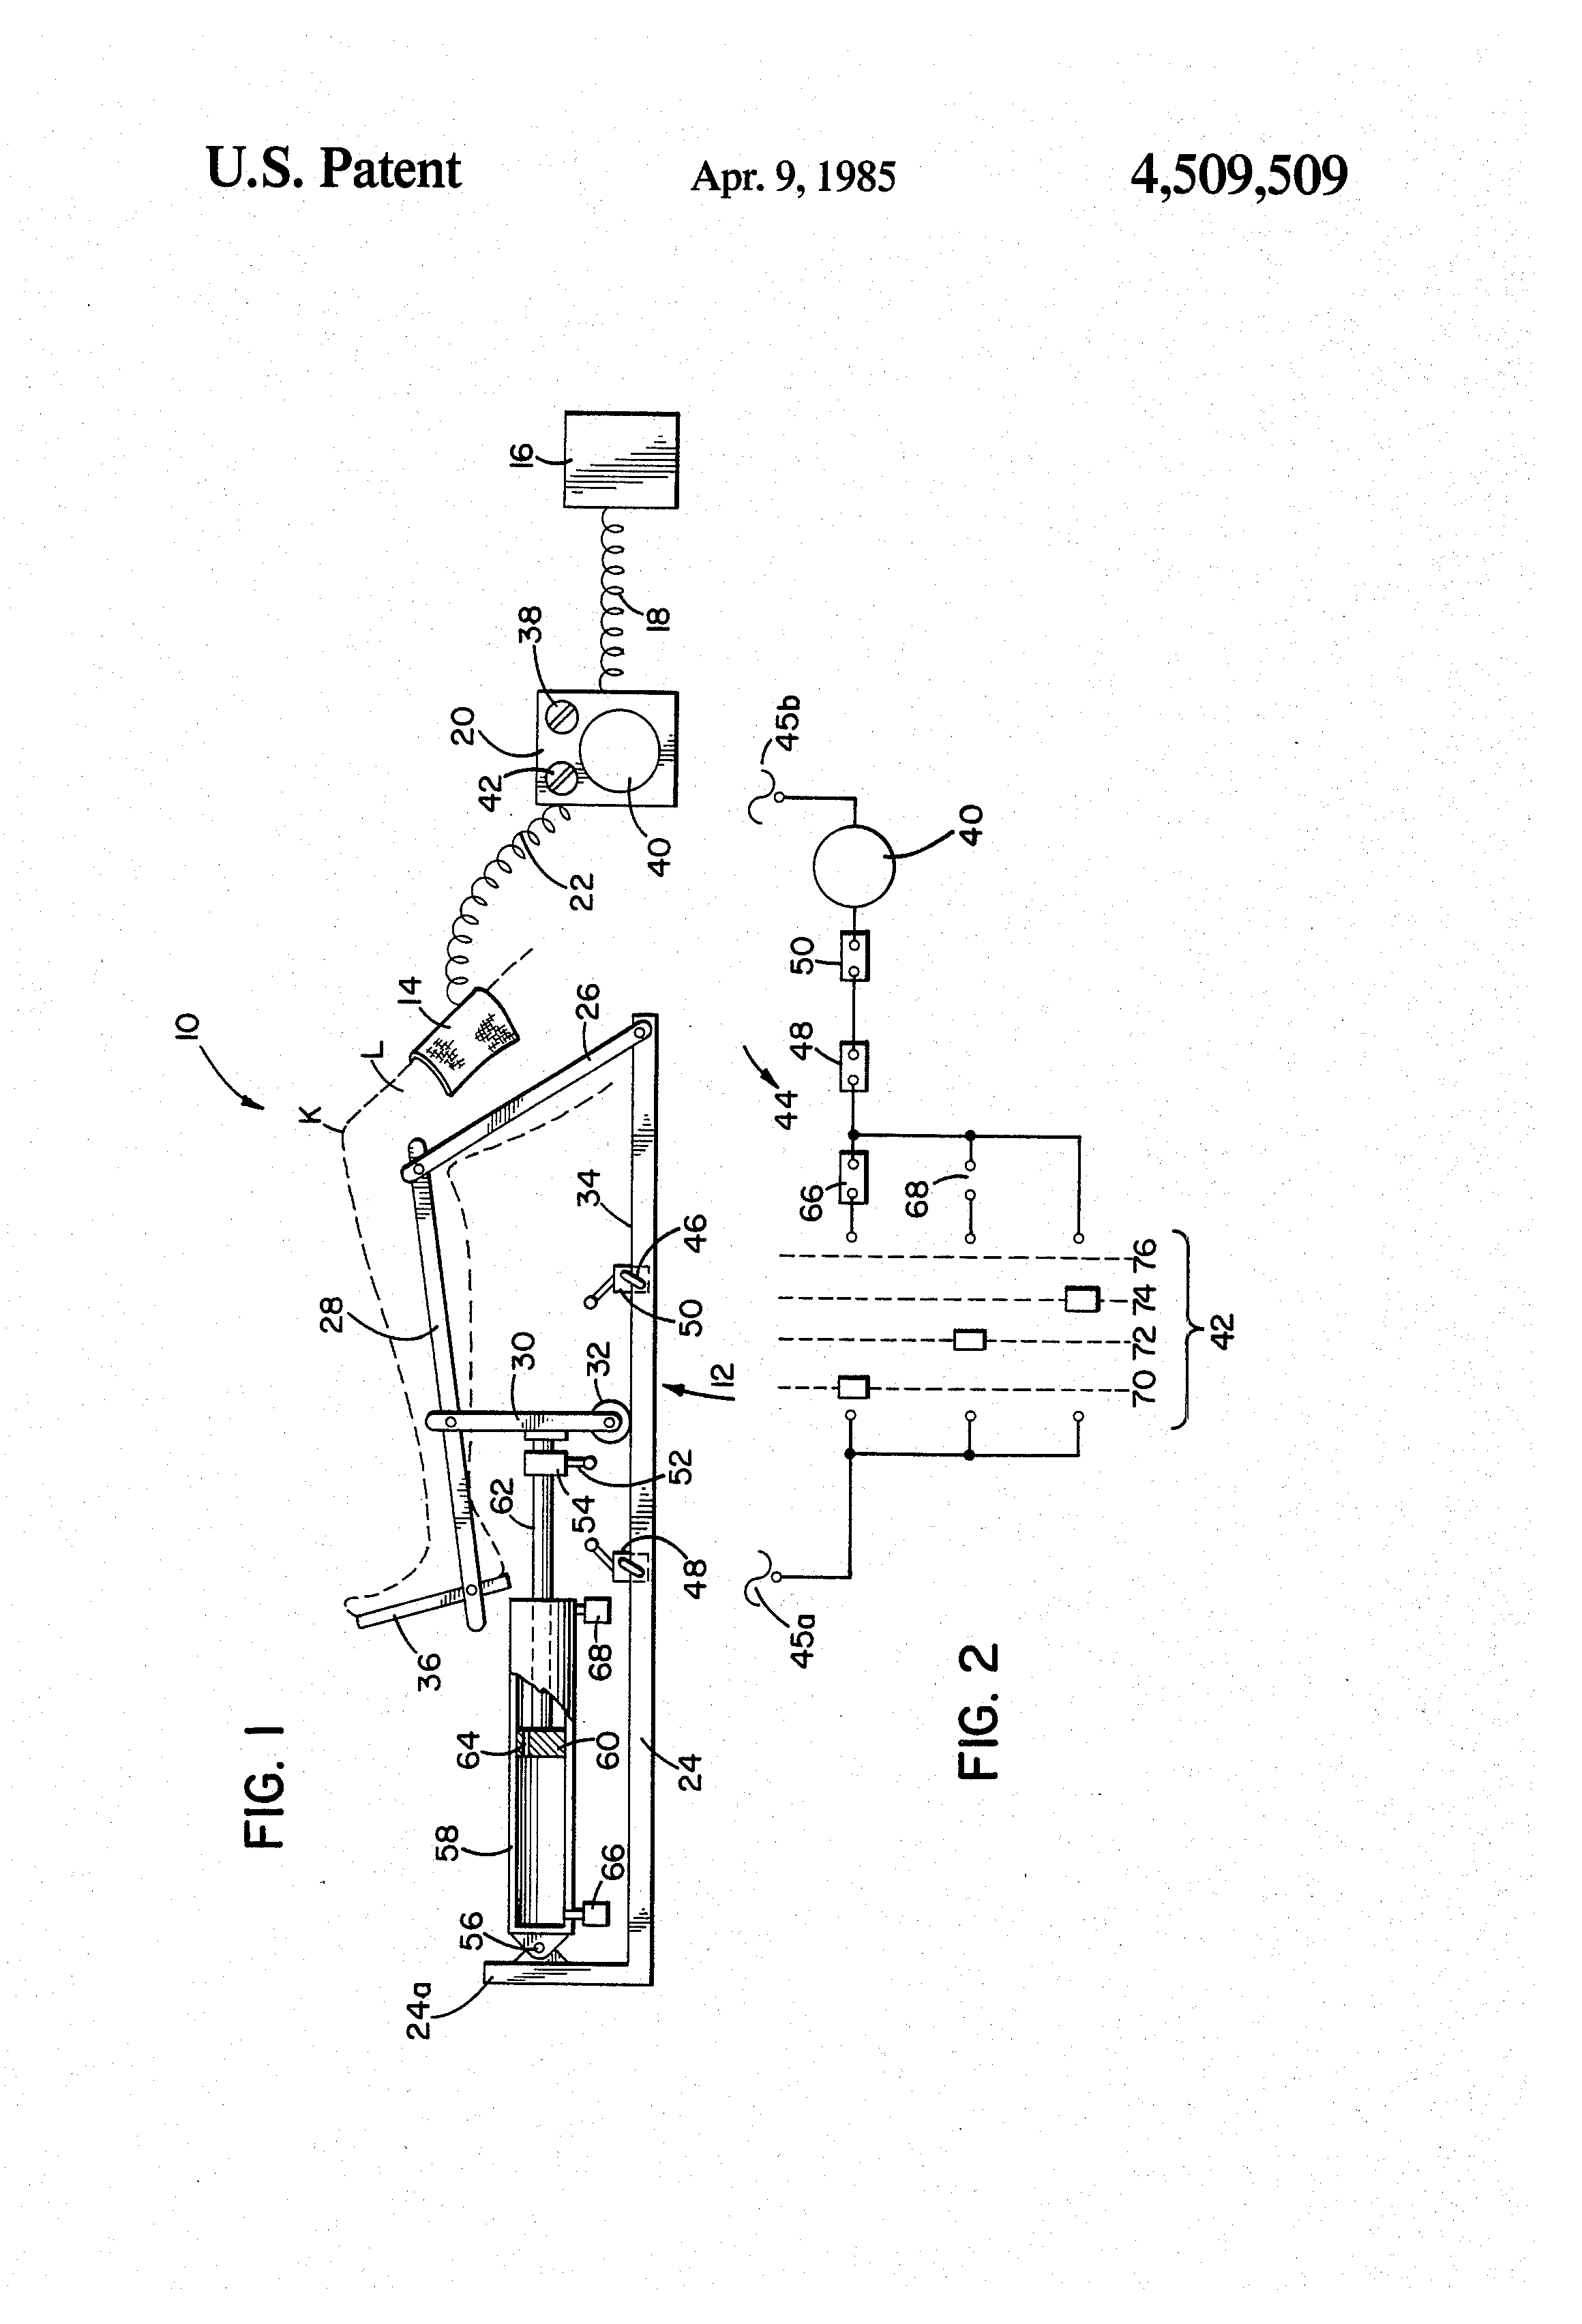
\includegraphics[width=0.54\linewidth]{US4509509.png}
  \caption{US4509509A apparatus illustrating adjustable thigh/calf supports and drive linkage.}
  \label{fig:US4509509A}
\end{figure}

\subsection{Mechanism kinematics}

\section{US4520827A: NMS Aided Continuous Passive Motion Apparatus}
\subsection{Description}
Integrates neuromuscular stimulation with CPM so electrical stimulation can be synchronized with passive motion. Aims to reduce atrophy and enhance neuromuscular re-education while maintaining safe, programmable knee motion profiles.
\subsection{Images}
\begin{figure}[H]
  \centering
  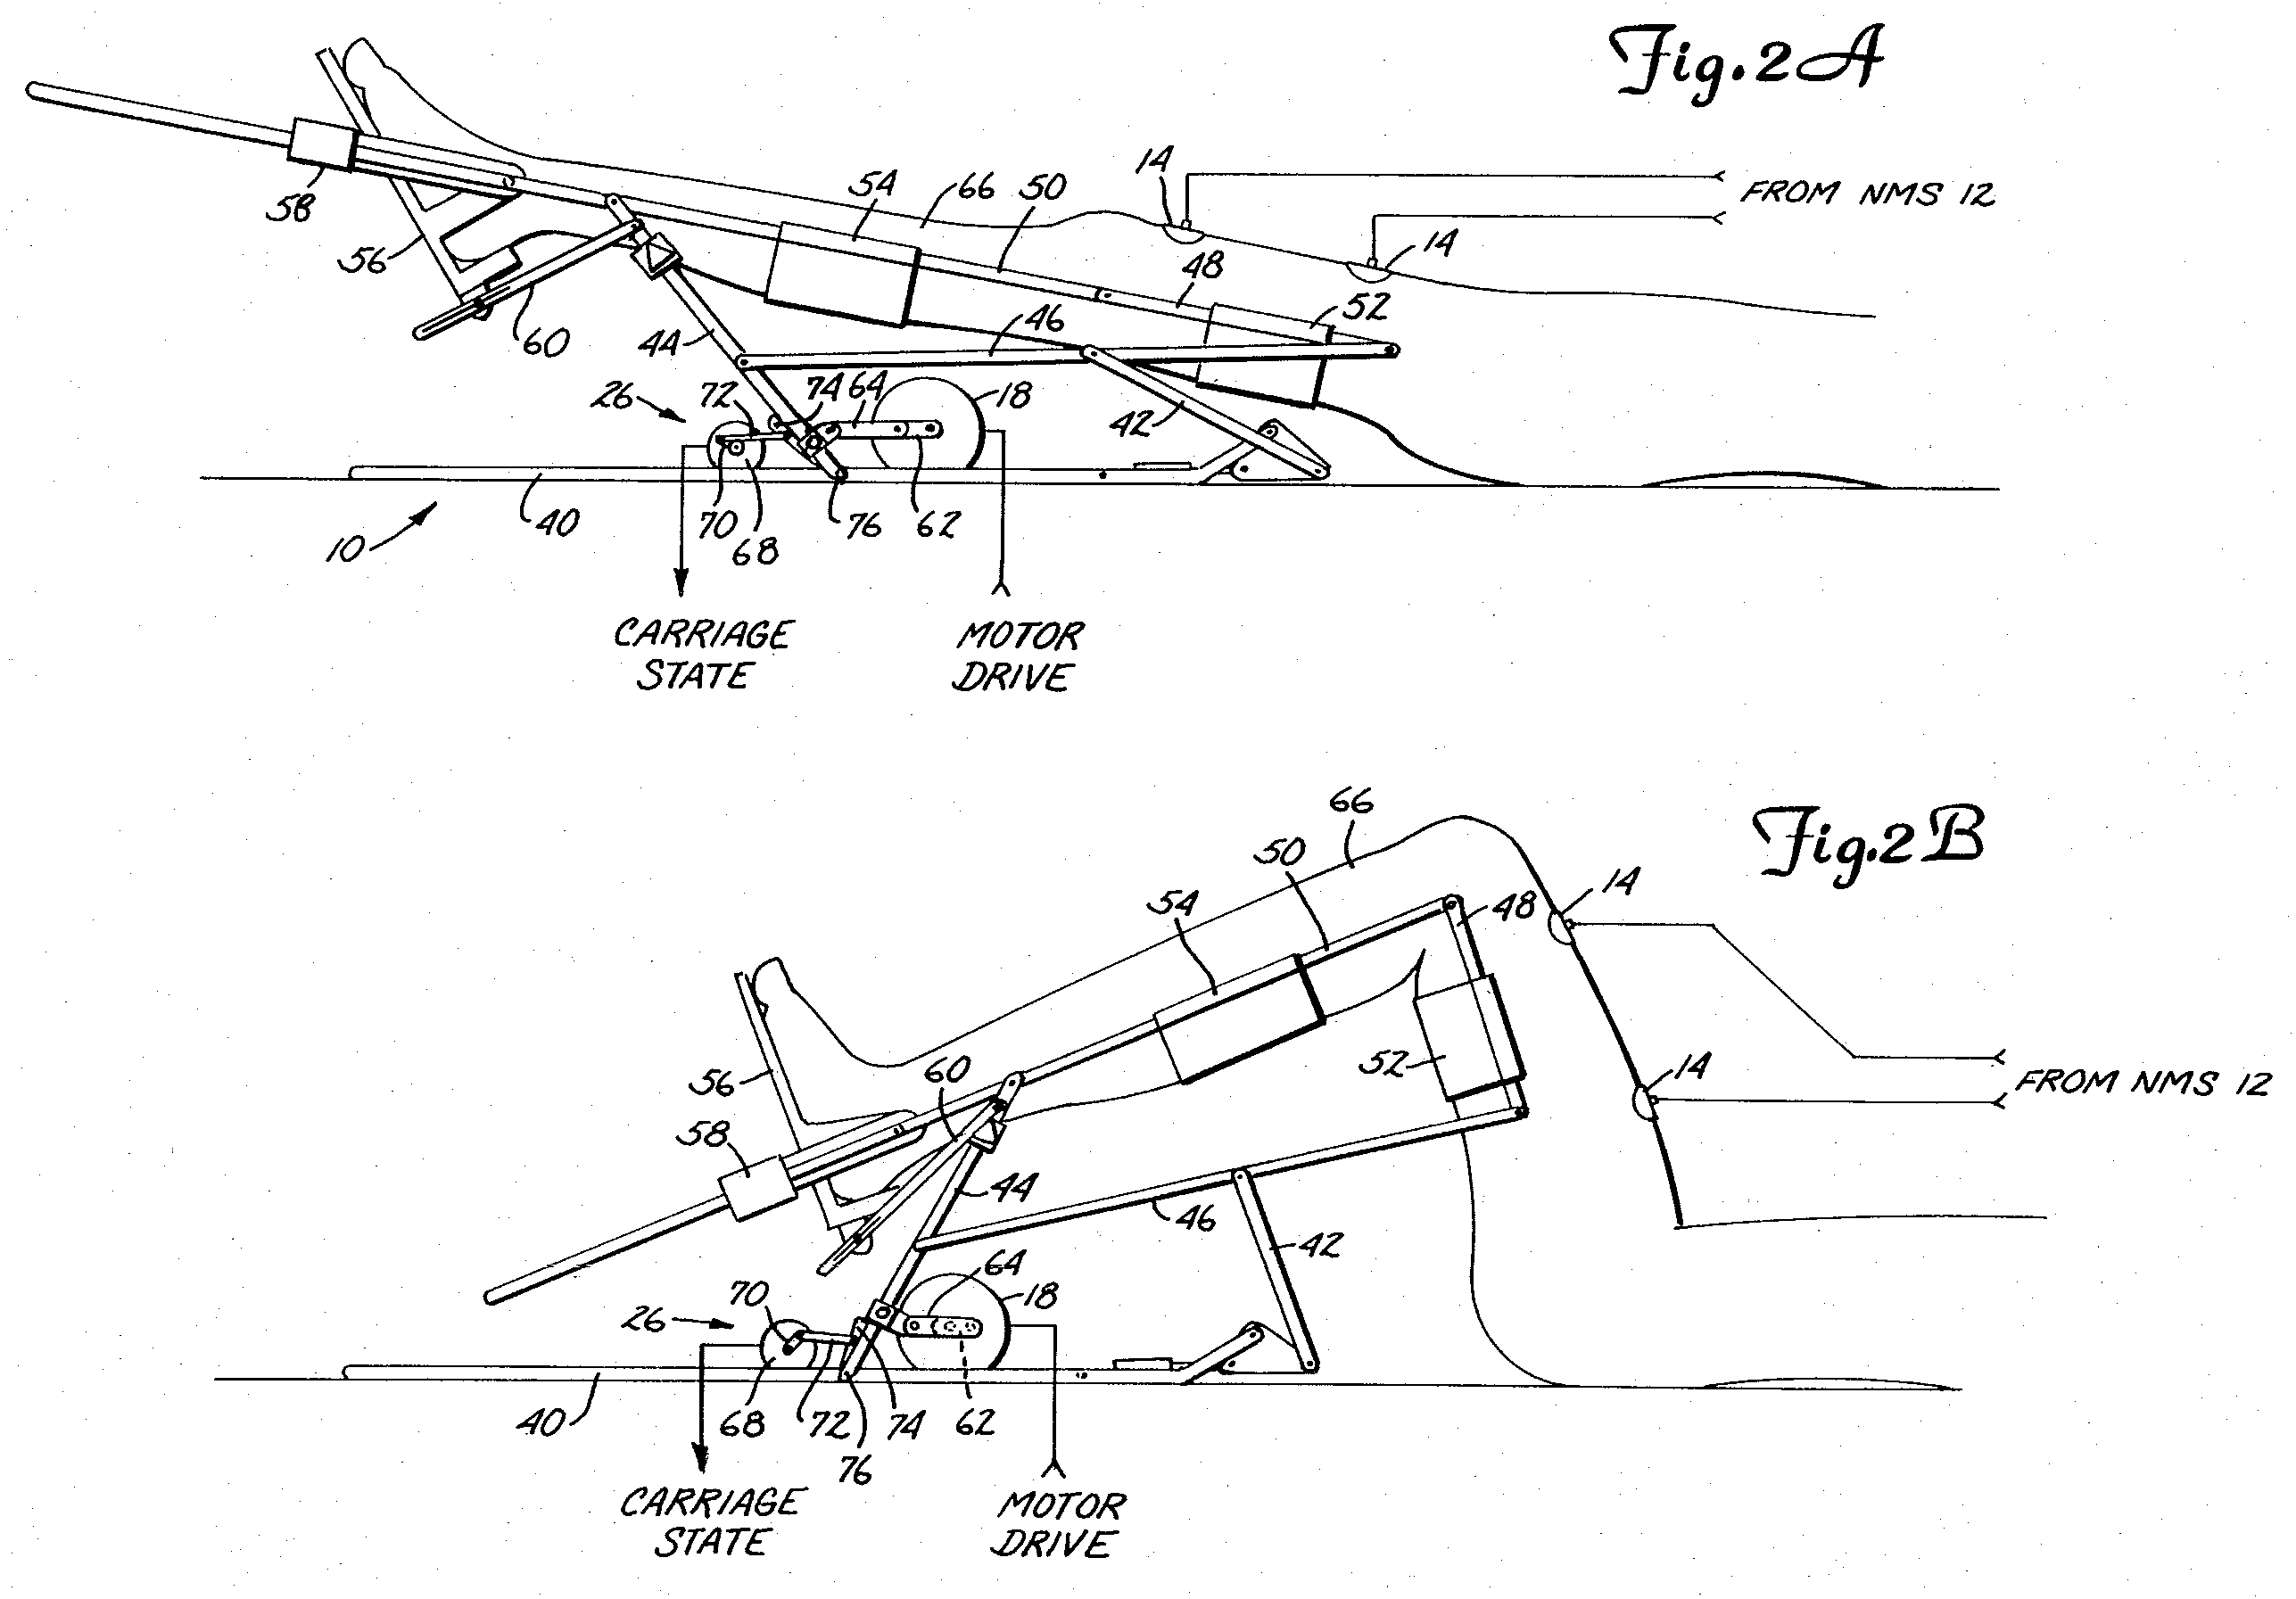
\includegraphics[width=0.54\linewidth]{US4520827.png}
  \caption{US4520827A concept combining CPM with synchronized neuromuscular stimulation.}
  \label{fig:US4520827A}
\end{figure}

\subsection{Mechanism kinematics}

\section{US4549534A: Leg Exercise Device}
\subsection{Description}
Compact leg exercise mechanism configured for passive knee cycling with an emphasis on home-use practicality. Utilizes a simple linkage and foot support to provide repeatable, low-load flexion/extension with minimal setup.
\subsection{Images}
\begin{figure}[H]
  \centering
  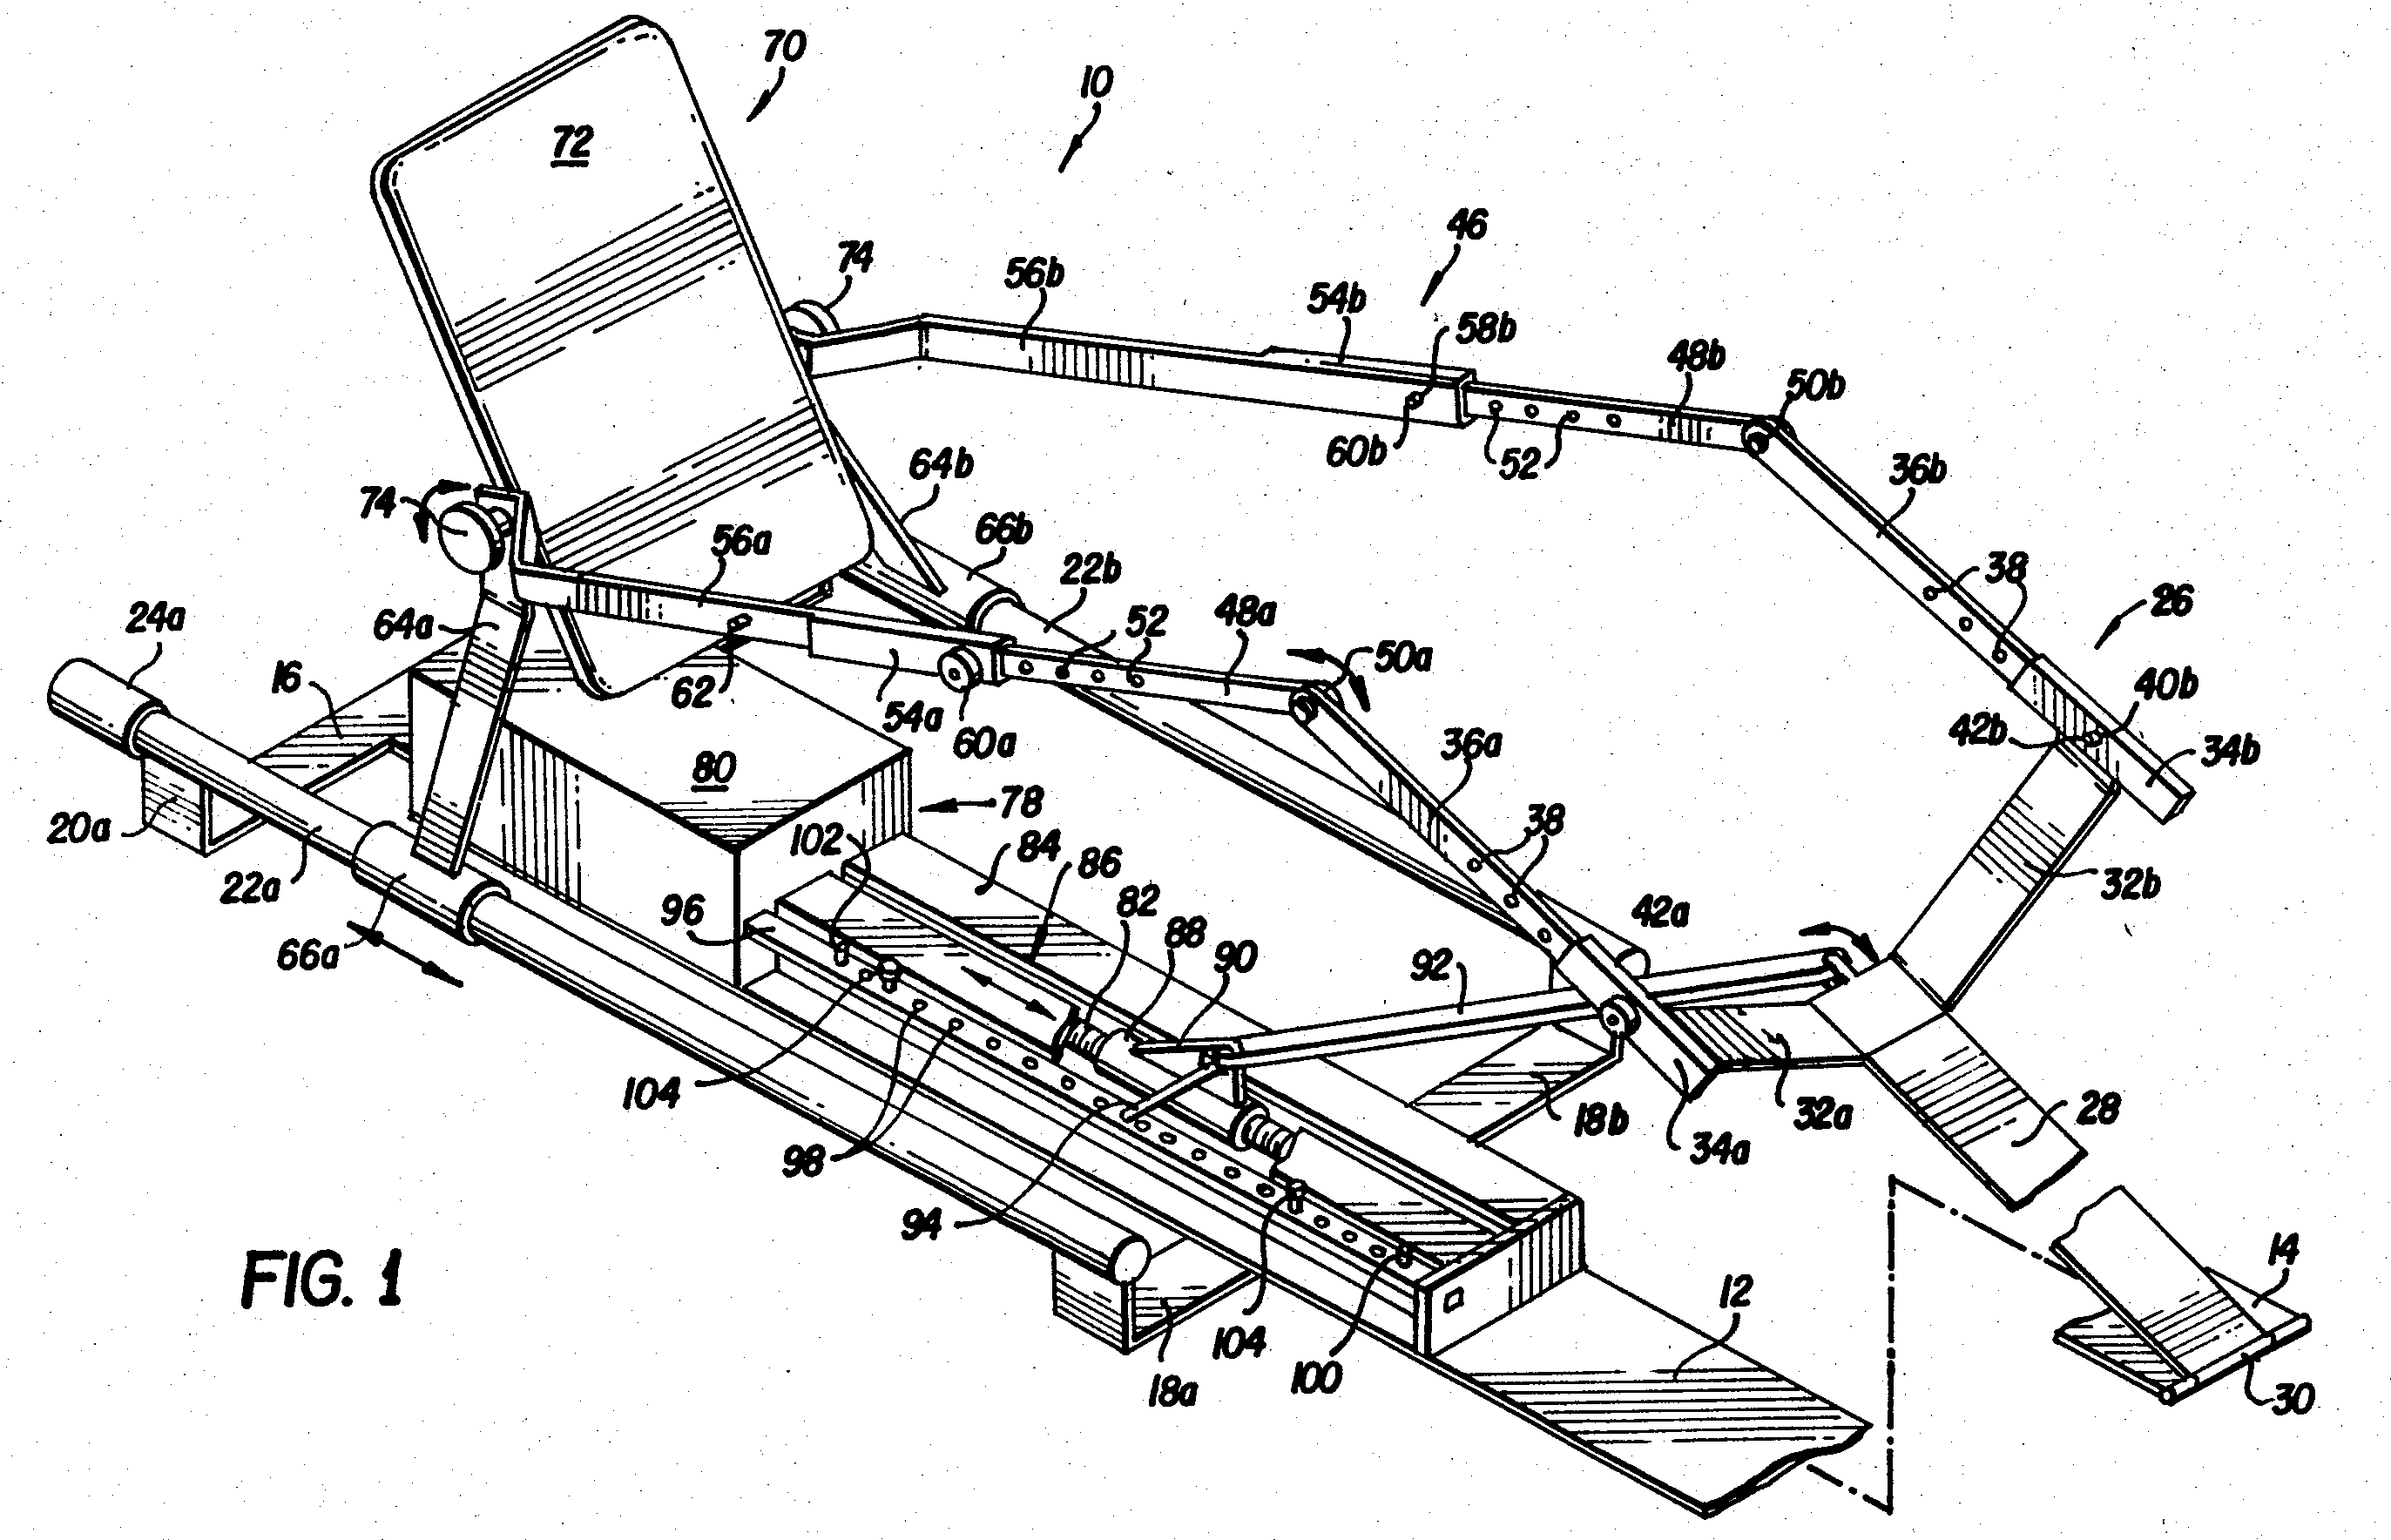
\includegraphics[width=0.54\linewidth]{US4549534.png}
  \caption{US4549534A leg exercise linkage aimed at repeatable passive motion.}
  \label{fig:US4549534A}
\end{figure}

\subsection{Mechanism kinematics}

\section{US4566440A: Orthosis for Leg Movement with Virtual Hip Pivot}
\subsection{Description}
Introduces a \emph{virtual hip pivot} to better replicate natural hip–knee kinematics during knee motion, reducing shear and improving alignment. The orthosis geometry helps maintain consistent joint axes throughout the CPM cycle.
\subsection{Images}
\begin{figure}[H]
  \centering
  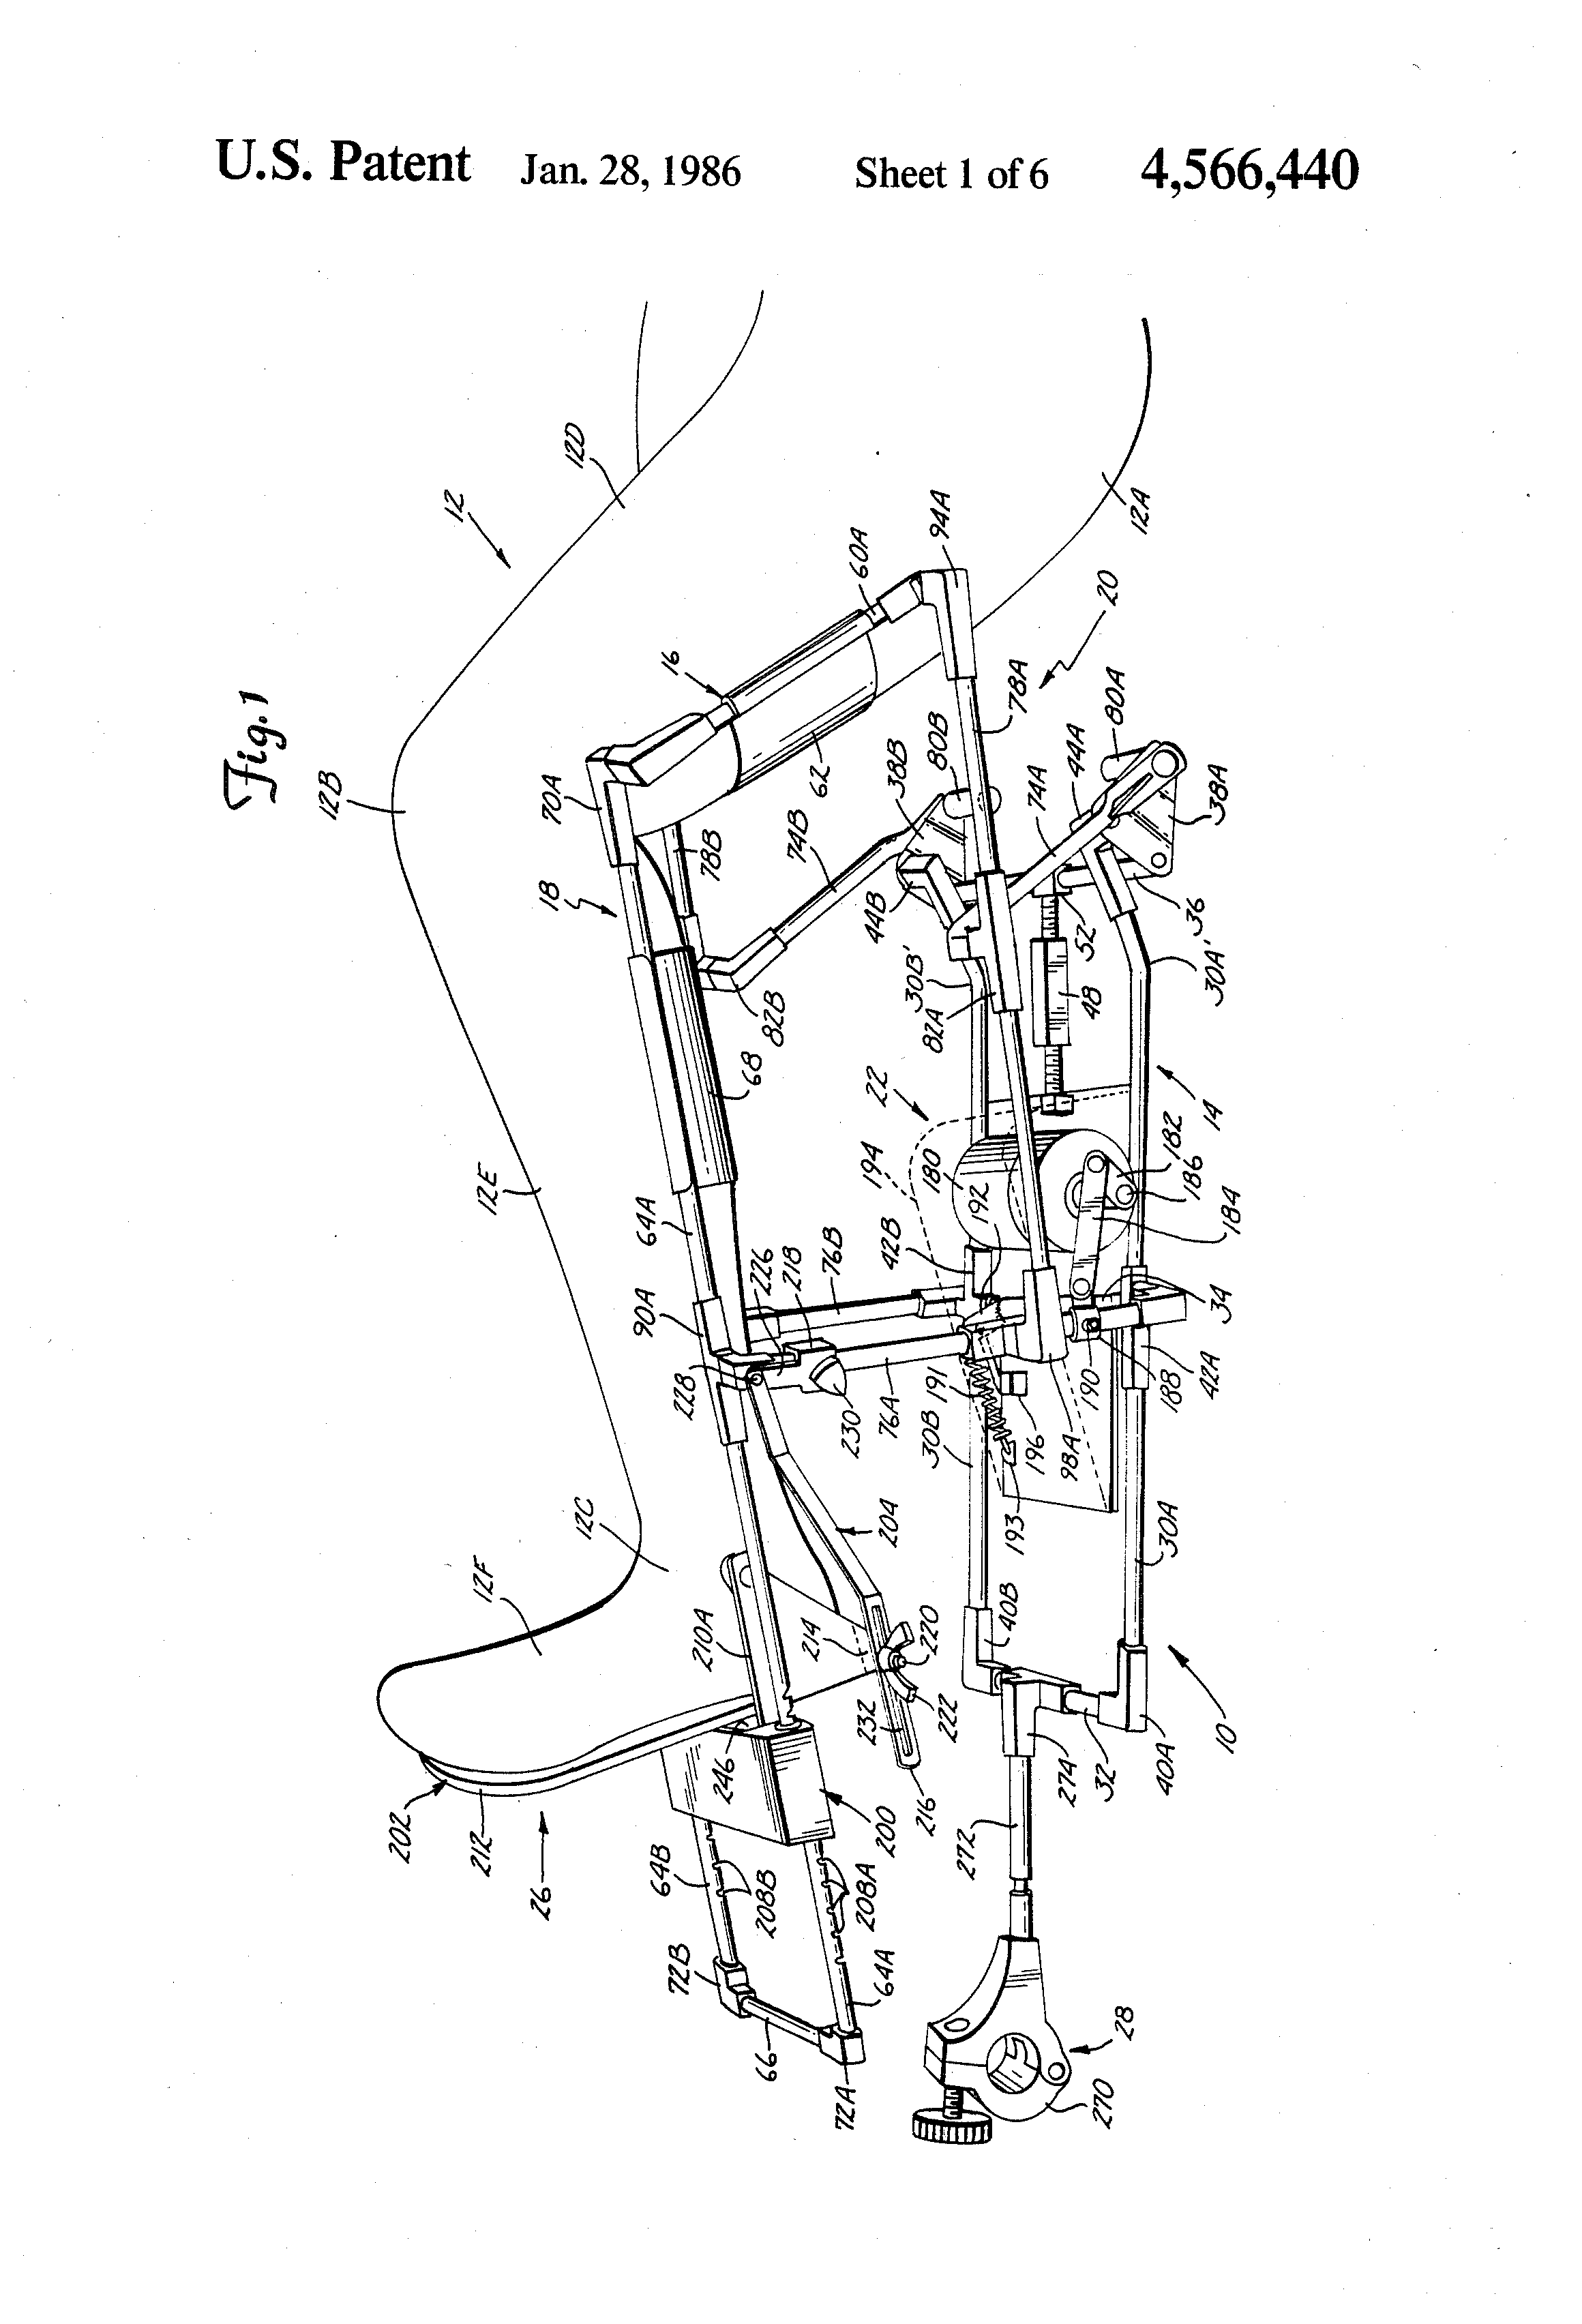
\includegraphics[width=0.54\linewidth]{US4566440_1.png}
  \caption{US4566440A orthosis showing geometry for a virtual hip pivot.}
  \label{fig:US4566440A}
\end{figure}

\subsection{Mechanism kinematics}

\section{US4974830A: Continuous Passive Motion Device}
\subsection{Description}
Programmable CPM with quick-adjust femoral and tibial cradles and mechanical end-stop management. Emphasizes user-friendly ROM adjustments and reliable actuator control for consistent therapy dosing.
\subsection{Images}
\begin{figure}[H]
  \centering
  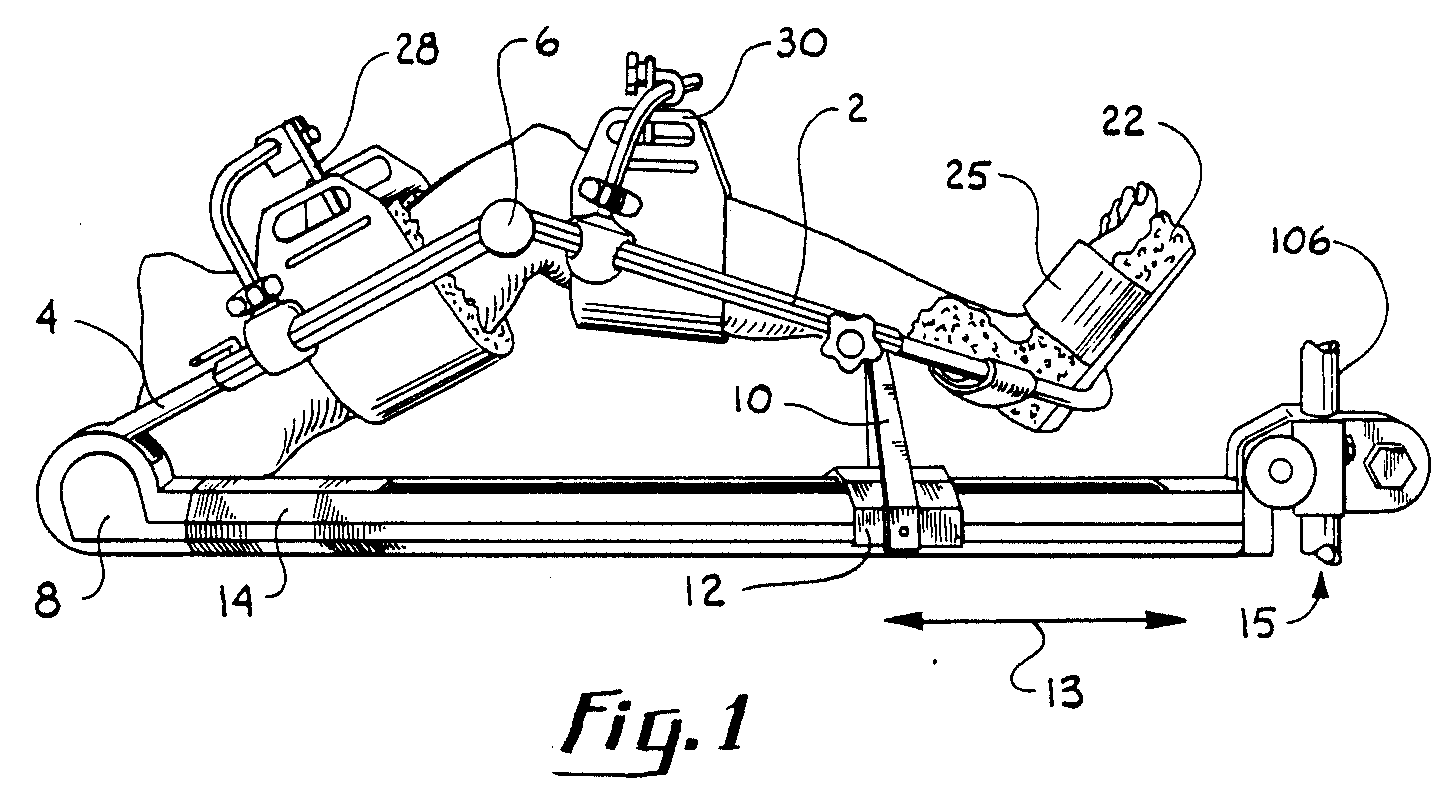
\includegraphics[width=0.54\linewidth]{US4974830_1.png}
  \caption{US4974830A CPM with adjustable cradles and end-stop control.}
  \label{fig:US4974830A}
\end{figure}

\subsection{Mechanism kinematics}

\section{US5203321A: Passive Anatomic Ankle–Foot Exerciser}
\subsection{Description}
Lower-limb passive motion device centered on anatomically aligned pivots and adjustable motion limits. Although focused on the ankle–foot complex, its design principles for alignment and controlled arcs inform knee CPM alignment strategies.
\subsection{Images}
\begin{figure}[H]
  \centering
  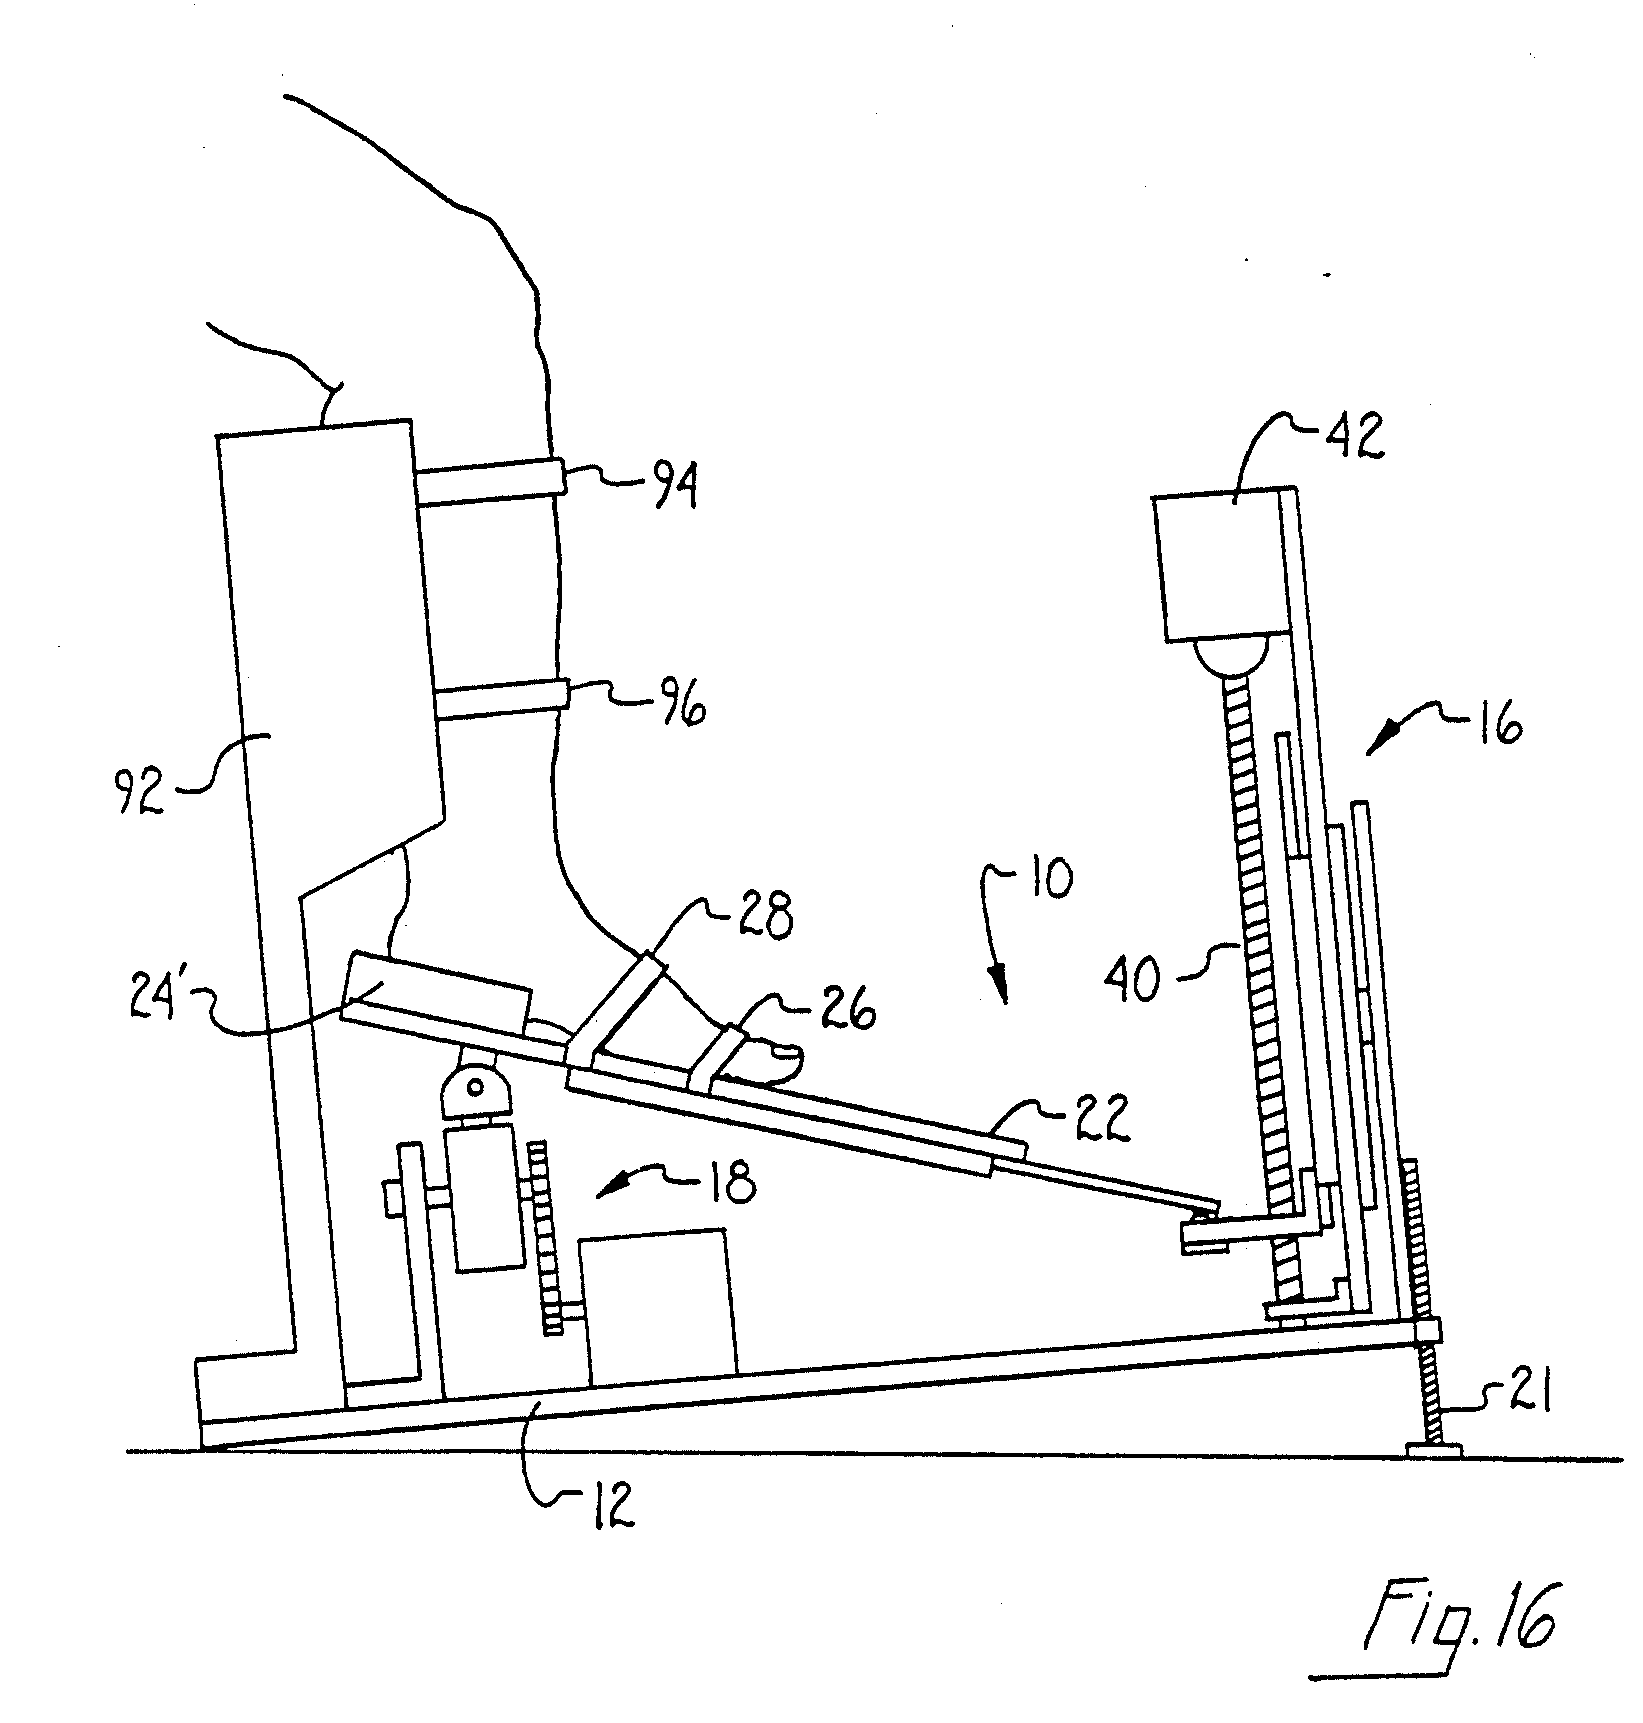
\includegraphics[width=0.54\linewidth]{US5203321_1.png}
  \caption{US5203321A passive device emphasizing anatomical pivot alignment.}
  \label{fig:US5203321A}
\end{figure}

\subsection{Mechanism kinematics}

\section{US5333604A: Patella Exercising Apparatus}
\subsection{Description}
Targets patellar tracking and anterior knee mechanics, providing controlled patellar motion and load pathways. Highlights isolated patellofemoral mobilization that can complement tibiofemoral CPM to address maltracking concerns.
\subsection{Images}
\begin{figure}[H]
  \centering
  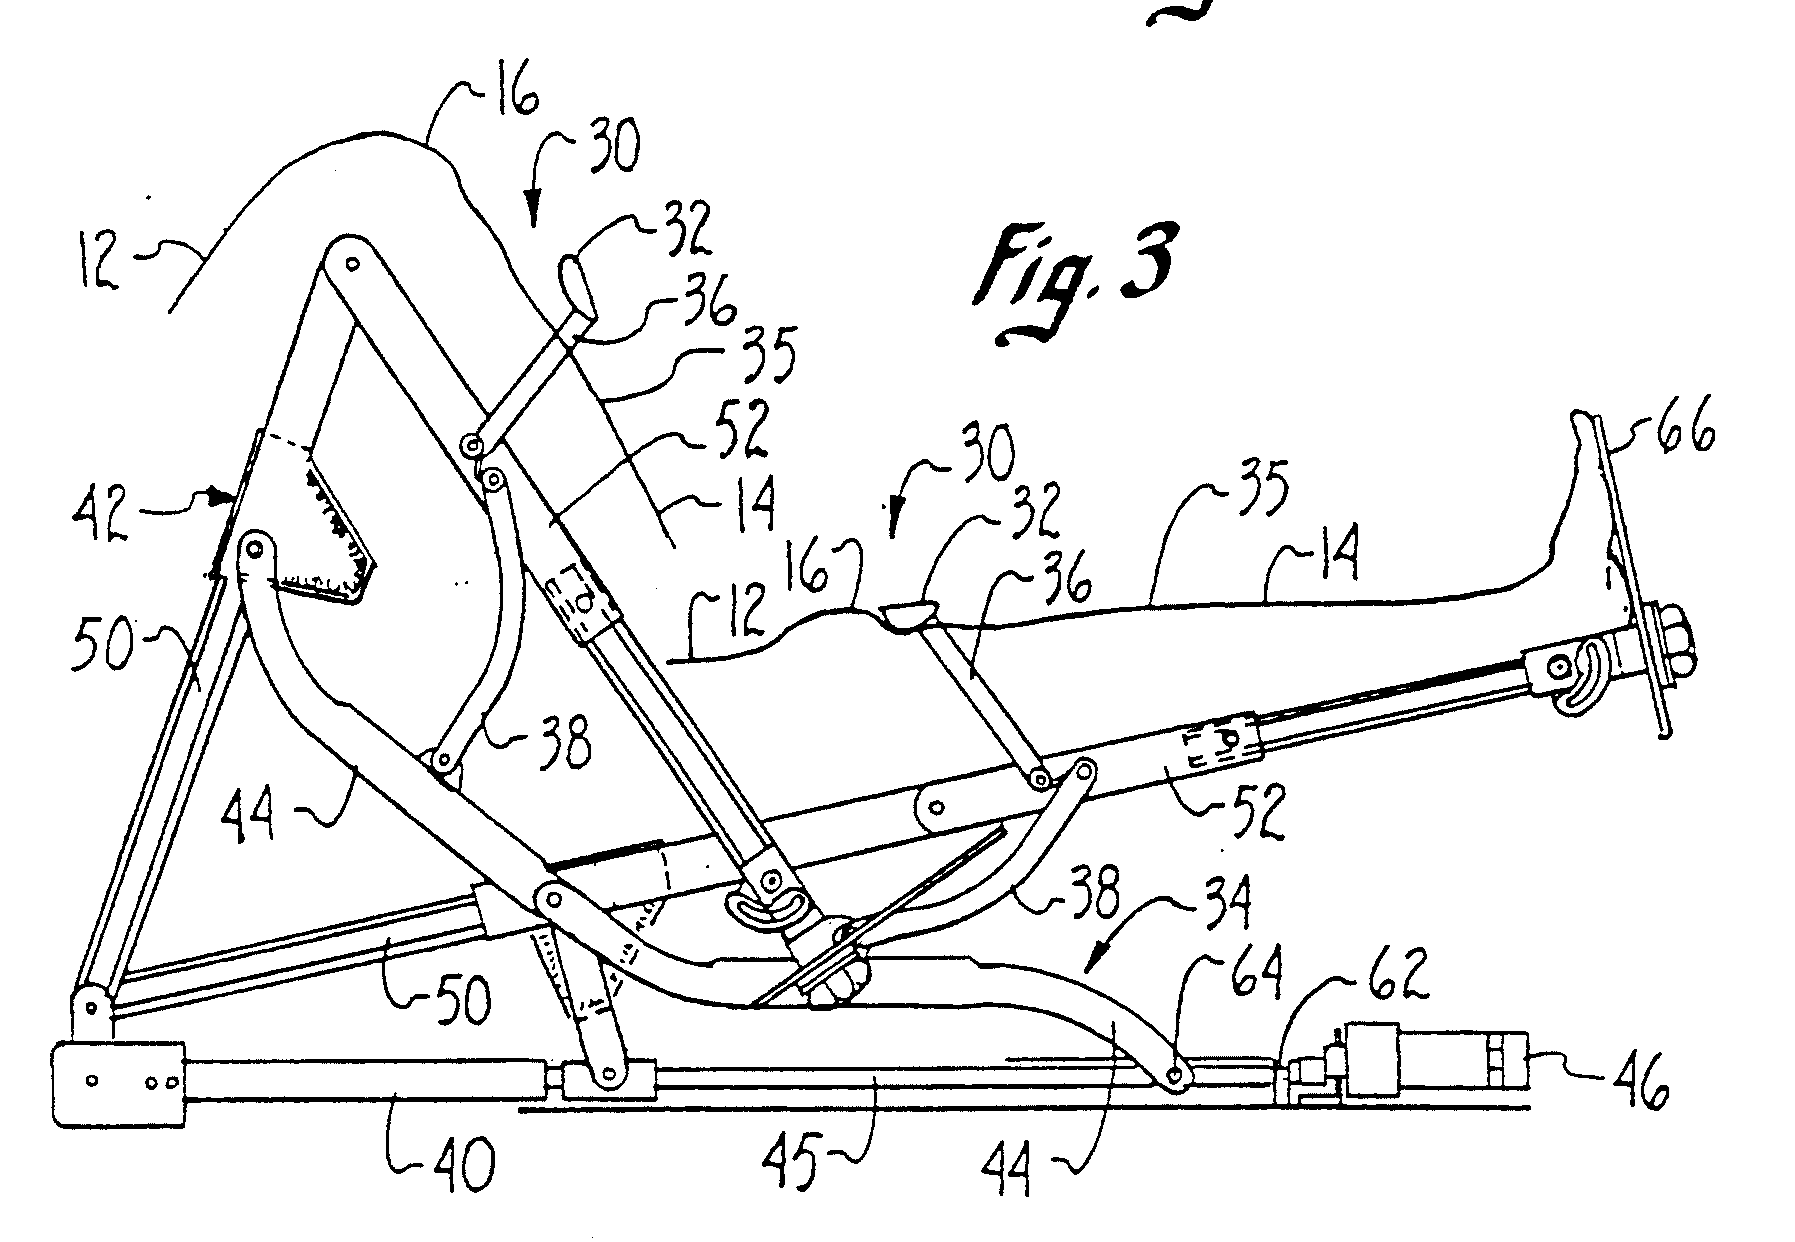
\includegraphics[width=0.54\linewidth]{US5333604_1.png}
  \caption{US5333604A apparatus for targeted patellar motion and tracking.}
  \label{fig:US5333604A}
\end{figure}

\subsection{Mechanism kinematics}

\section{US6267735B1: Continuous Passive Motion Device Having a Comfort Zone Feature}
\subsection{Description}
Implements a \emph{comfort zone} deadband that avoids painful end ranges by adapting speed or reversing before irritation thresholds. Designed to increase tolerance and session duration while preserving therapeutic ROM gains.
\subsection{Images}
\begin{figure}[H]
  \centering
  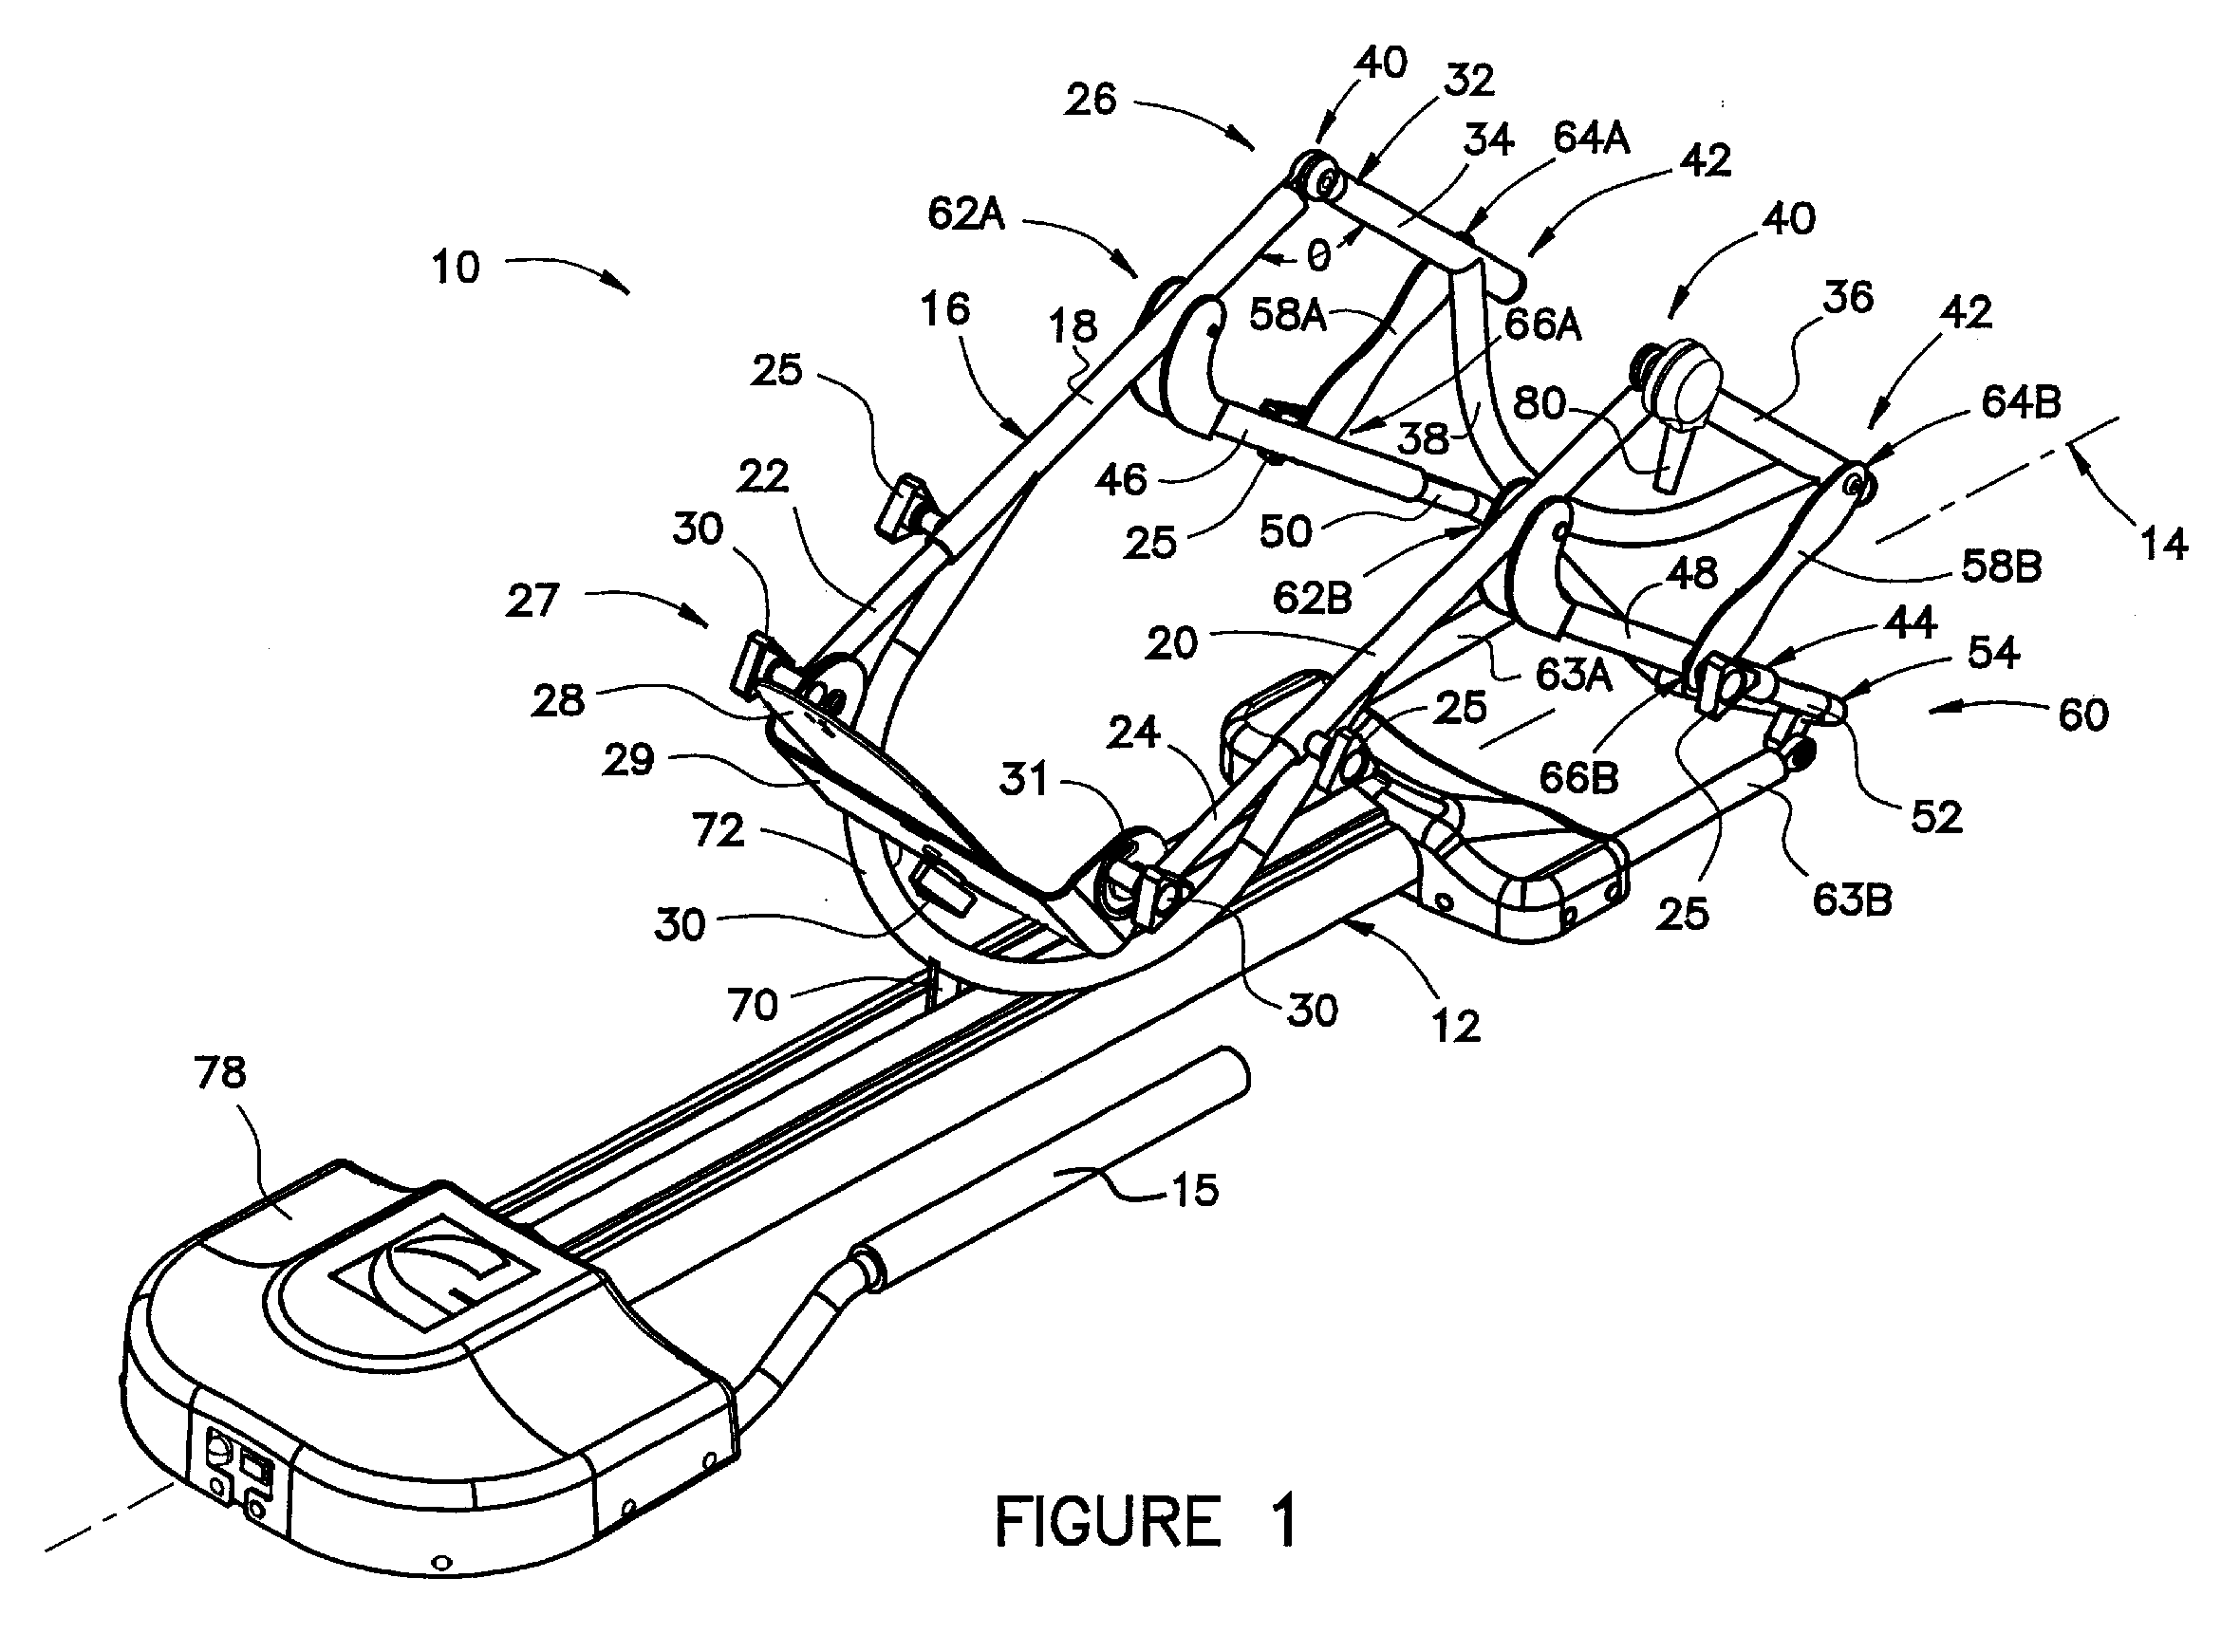
\includegraphics[width=0.54\linewidth]{US6267735B1_1.png}
  \caption{US6267735B1 CPM featuring an adaptive comfort-zone deadband.}
  \label{fig:US6267735B1}
\end{figure}

\subsection{Mechanism kinematics}

\section{US6325770B1: Device for Producing Continuous Passive Motion}
\subsection{Description}
Mechanical drive (e.g., cam/gear) tuned to follow a knee-like path, aiming for physiologic tibiofemoral motion. Focuses on smooth kinematics and robust transmission to reduce backlash and improve comfort.
\subsection{Images}
\begin{figure}[H]
  \centering
  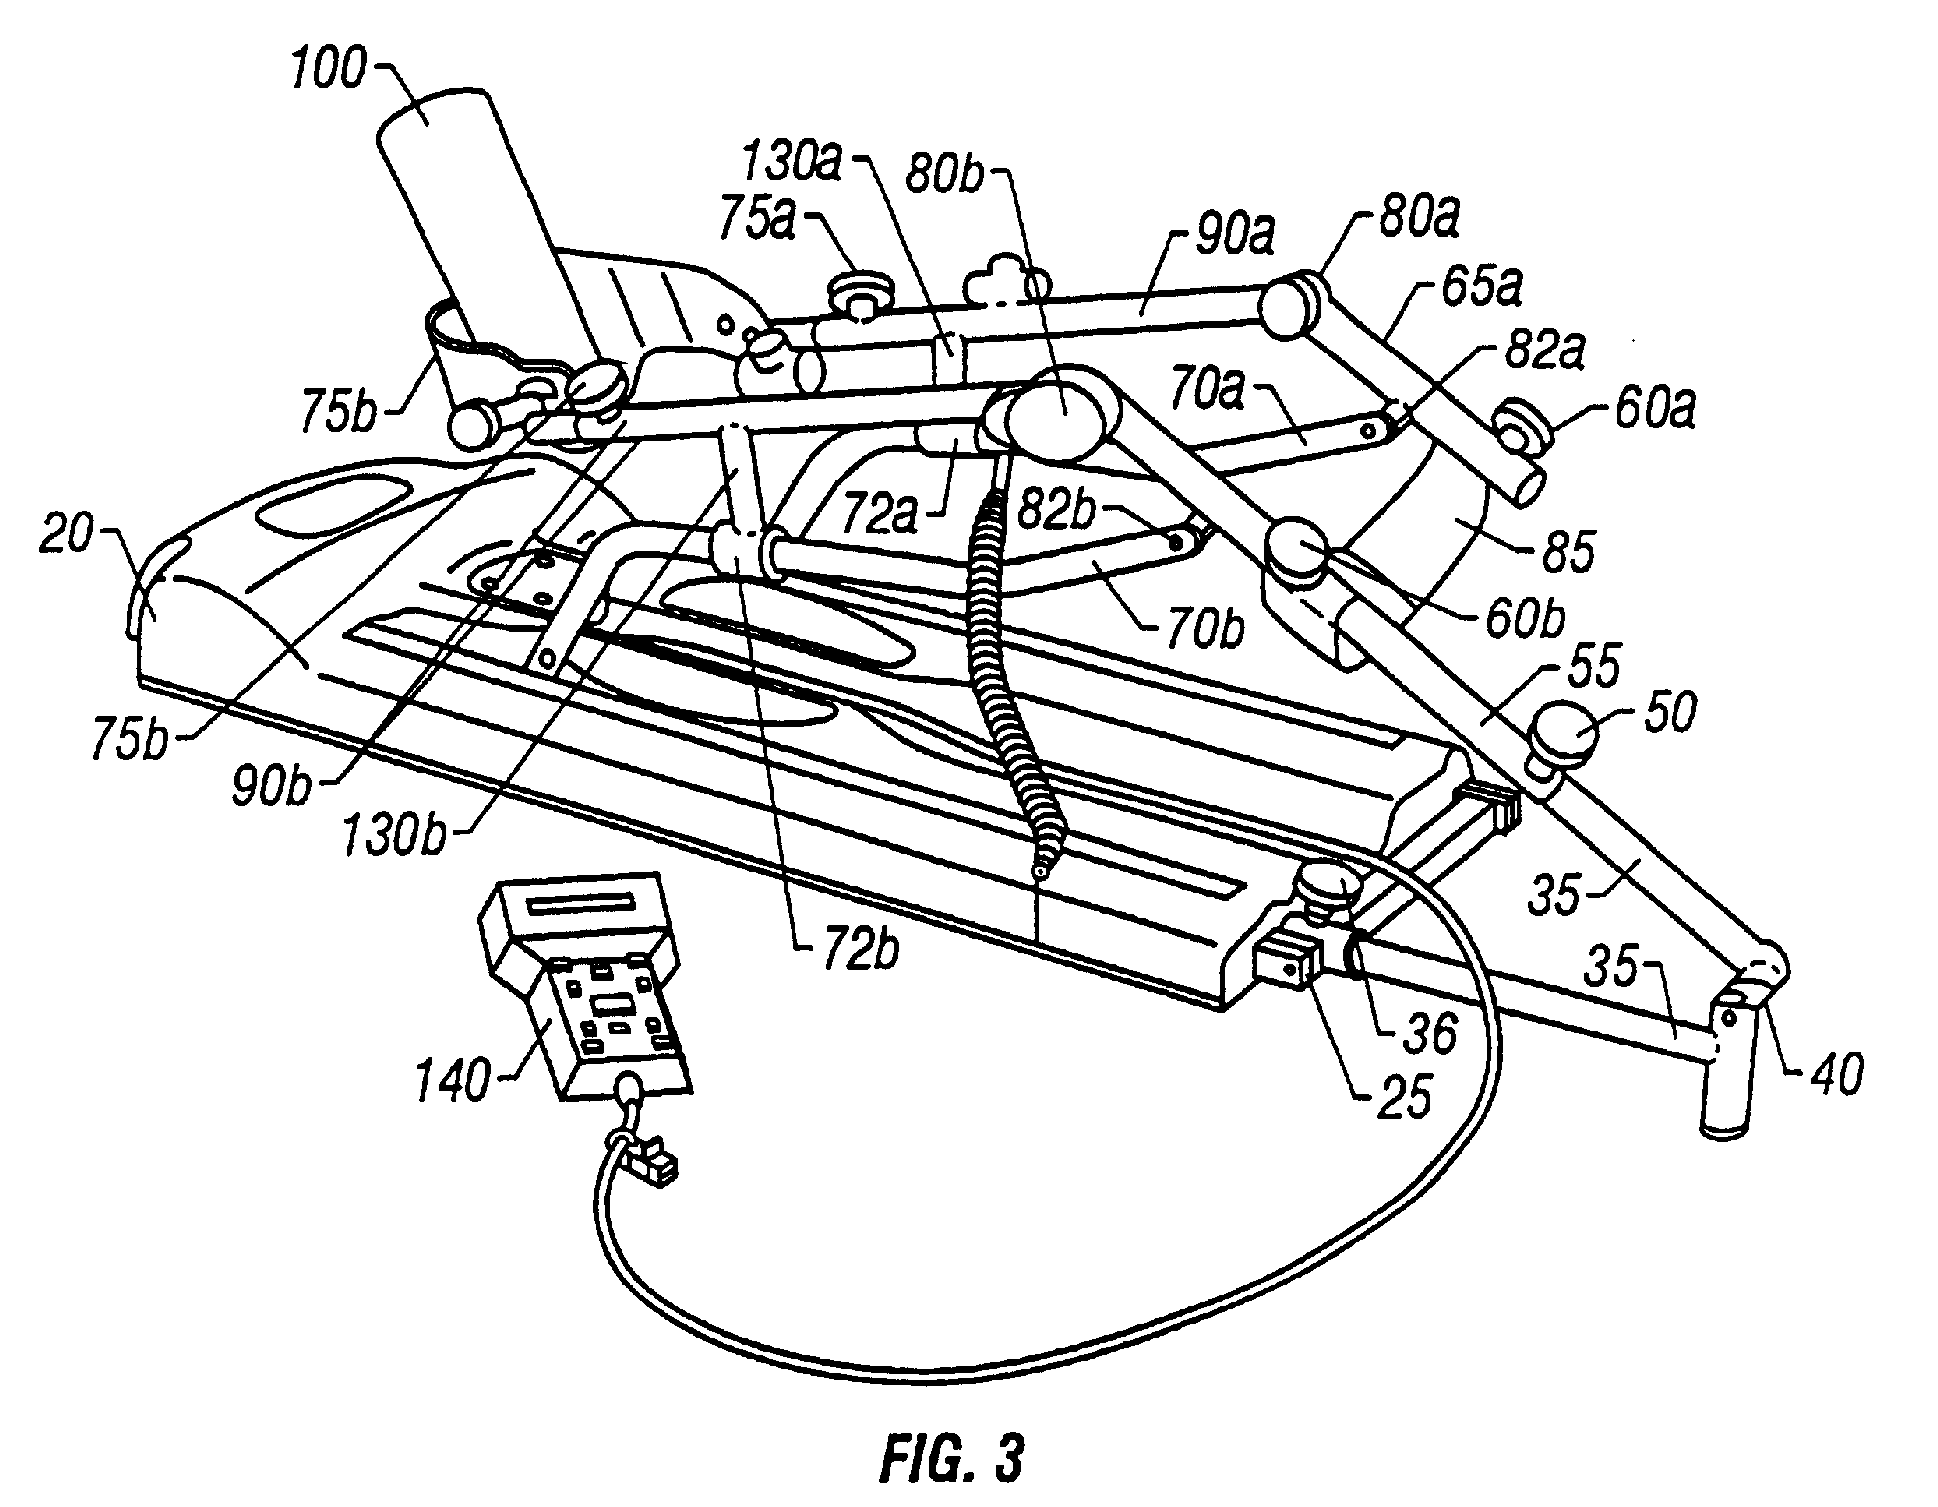
\includegraphics[width=0.54\linewidth]{US6325770B1_1.png}
  \caption{US6325770B1 transmission tuned for knee-like motion paths.}
  \label{fig:US6325770B1}
\end{figure}

\subsection{Mechanism kinematics}

\section{US5252102A: Electronic Range of Motion Apparatus for Orthosis/Prosthesis/CPM}
\subsection{Description}
Integrates electronic ROM sensing and feedback into an orthotic/CPM framework. Enables measurement-driven progression, alarms for unsafe limits, and data logging for clinical assessment.
\subsection{Images}
\begin{figure}[H]
  \centering
  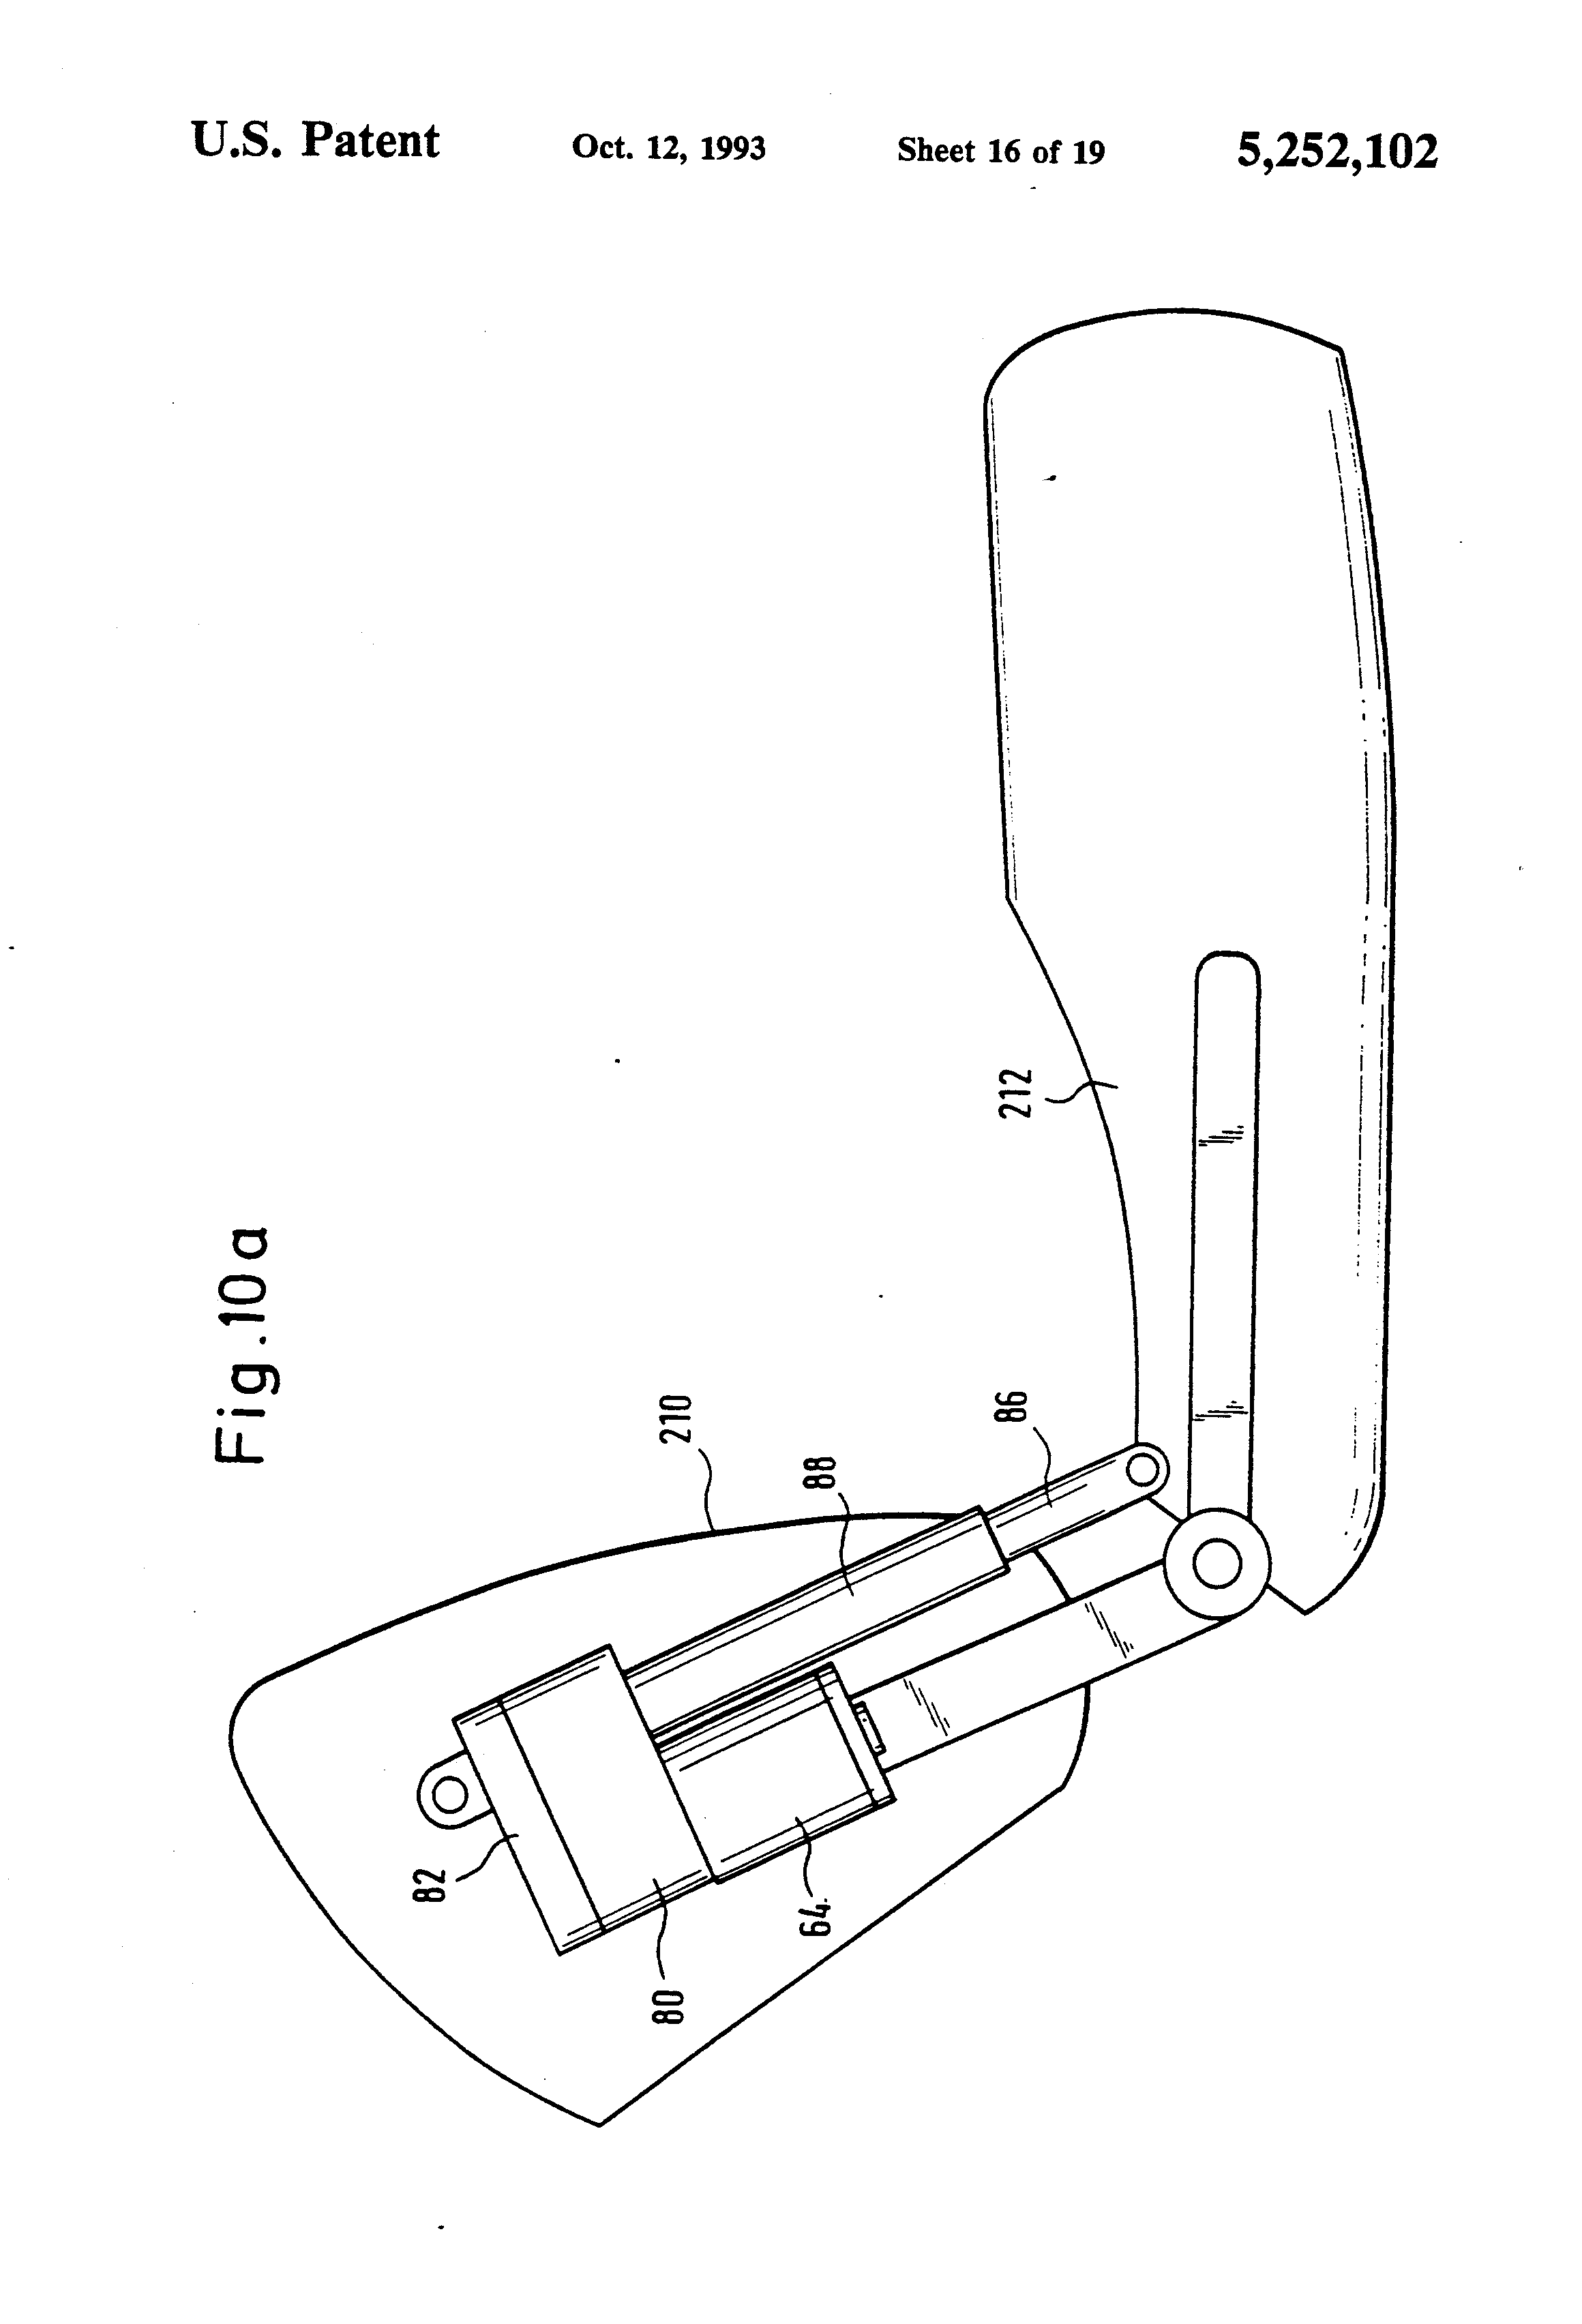
\includegraphics[width=0.54\linewidth]{US5252102_1.png}
  \caption{US5252102A apparatus with integrated electronic ROM sensing.}
  \label{fig:US5252102A}
\end{figure}

\subsection{Mechanism kinematics}

\section{US5280783A: Continuous Passive Motion Device for Full Extension of Leg}
\subsection{Description}
Prioritizes achieving and maintaining full knee extension with adjustable extension bias and end-range control. Useful for post-operative protocols where extension deficits are common.
\subsection{Images}
\begin{figure}[H]
  \centering
  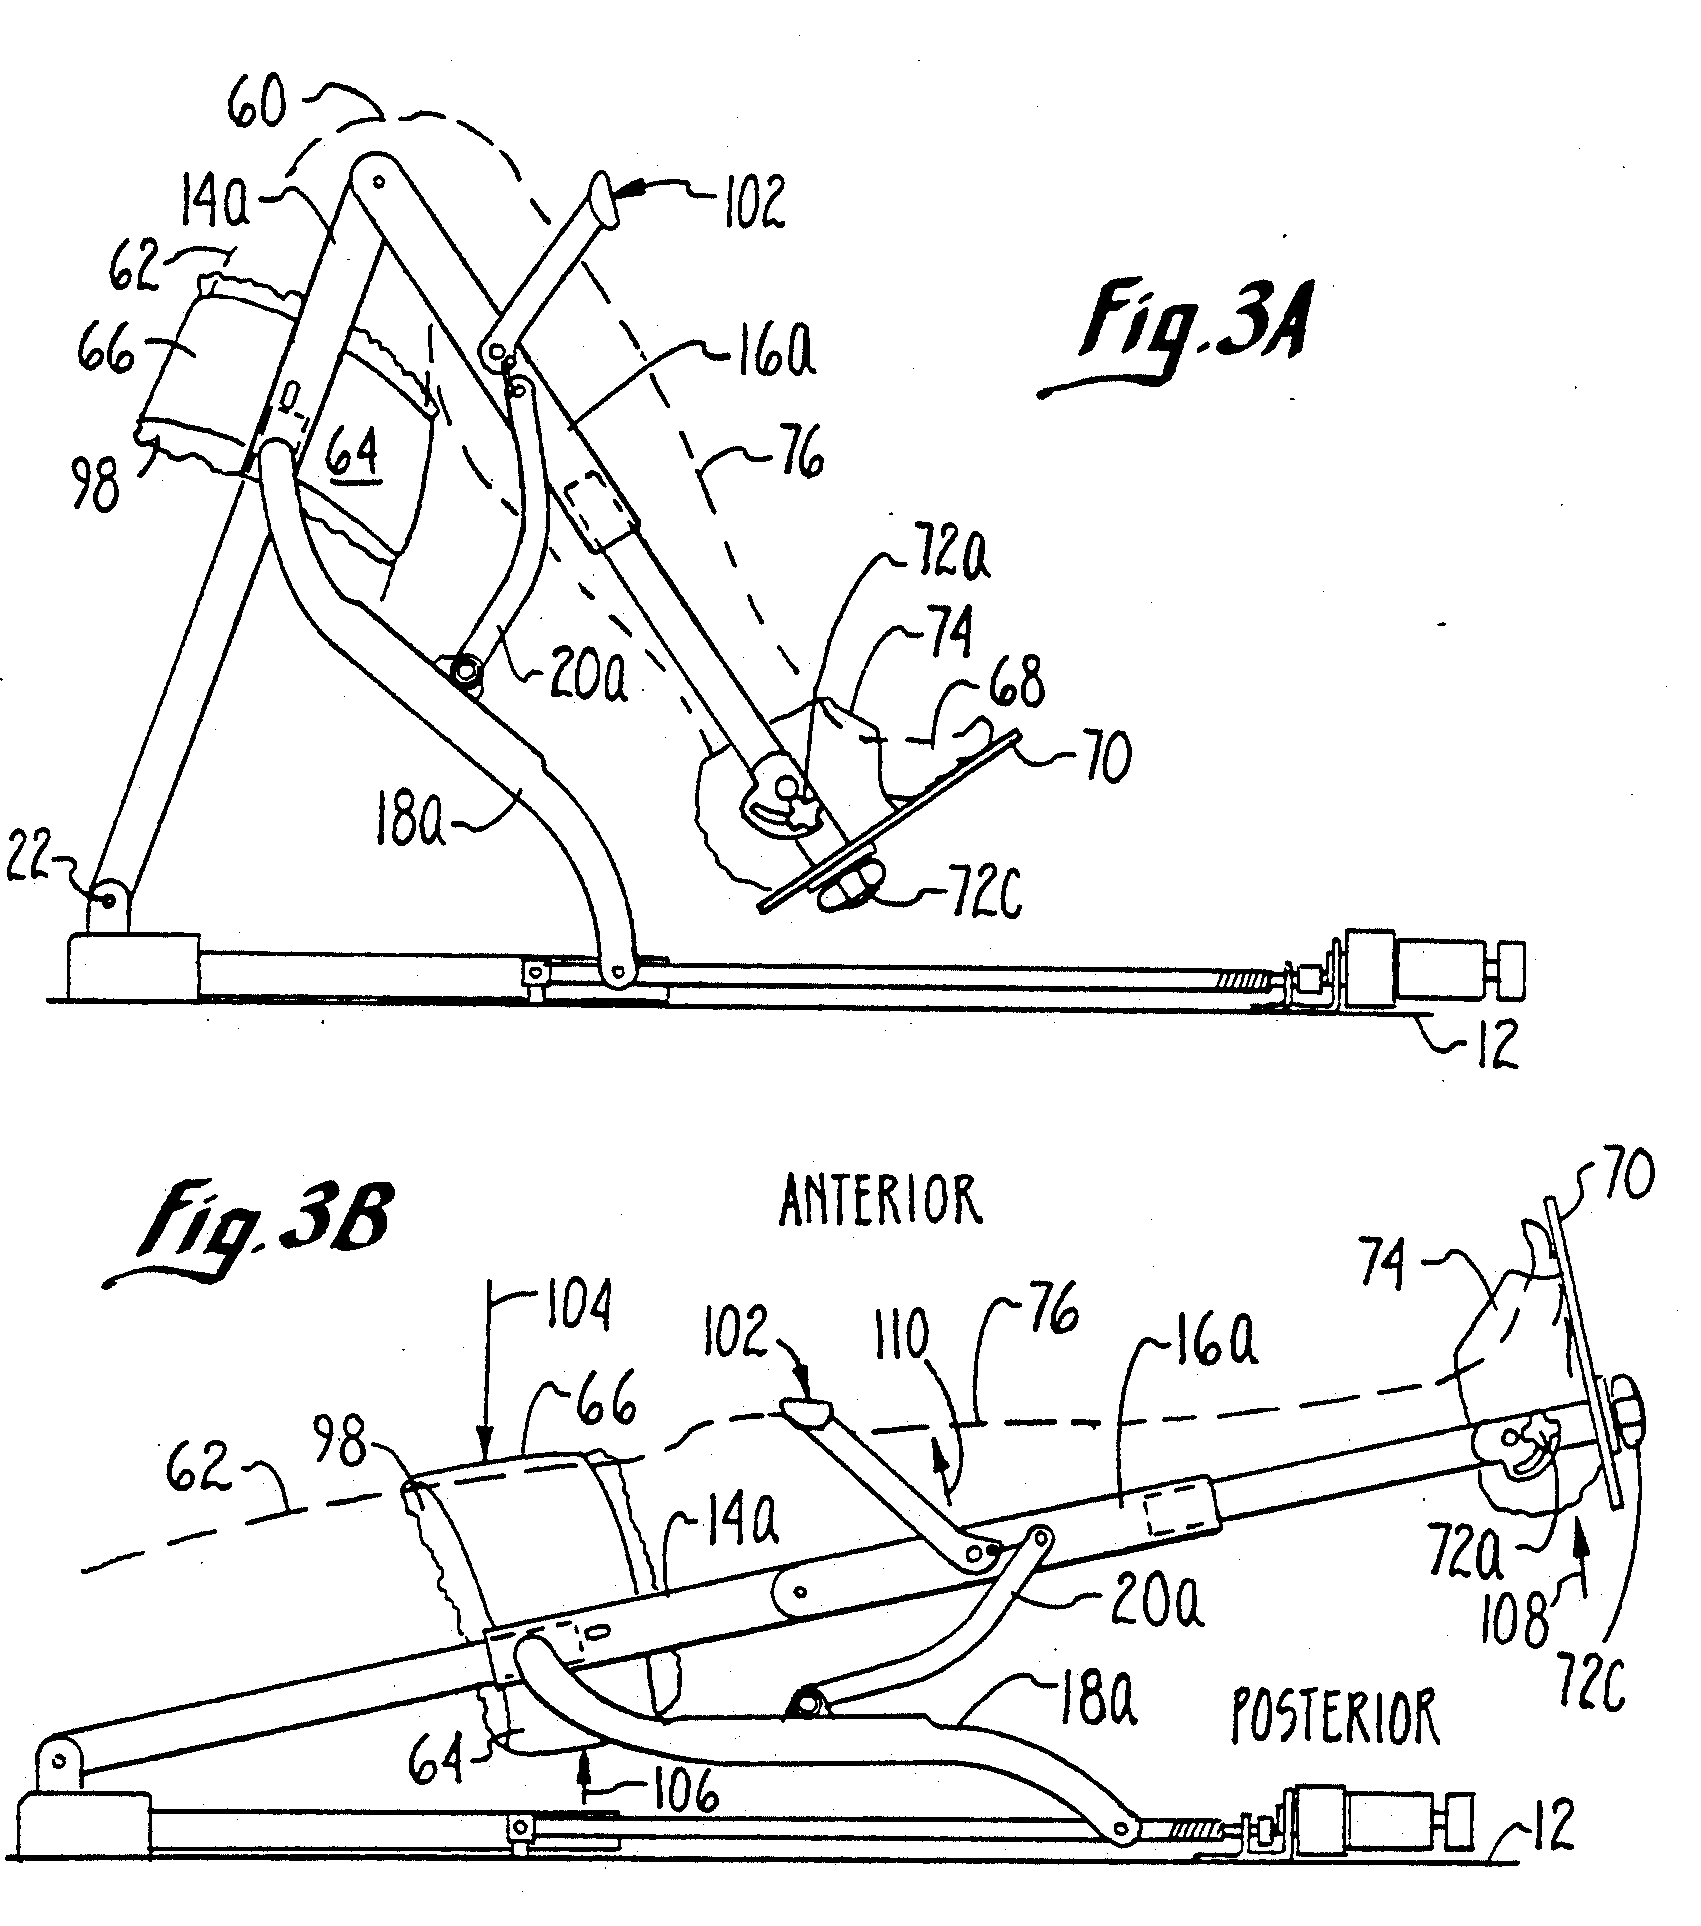
\includegraphics[width=0.54\linewidth]{US5280783_1.png}
  \caption{US5280783A CPM emphasizing controlled full-extension capability.}
  \label{fig:US5280783A}
\end{figure}

\subsection{Mechanism kinematics}

\section{US4492222A: Knee Exercise Machine}
\subsection{Description}
Adjustable axis alignment between femoral and tibial supports with a stable footplate to promote consistent knee pivoting. Emphasizes structural simplicity and robust construction for repeated clinical use.
\subsection{Images}
\begin{figure}[H]
  \centering
  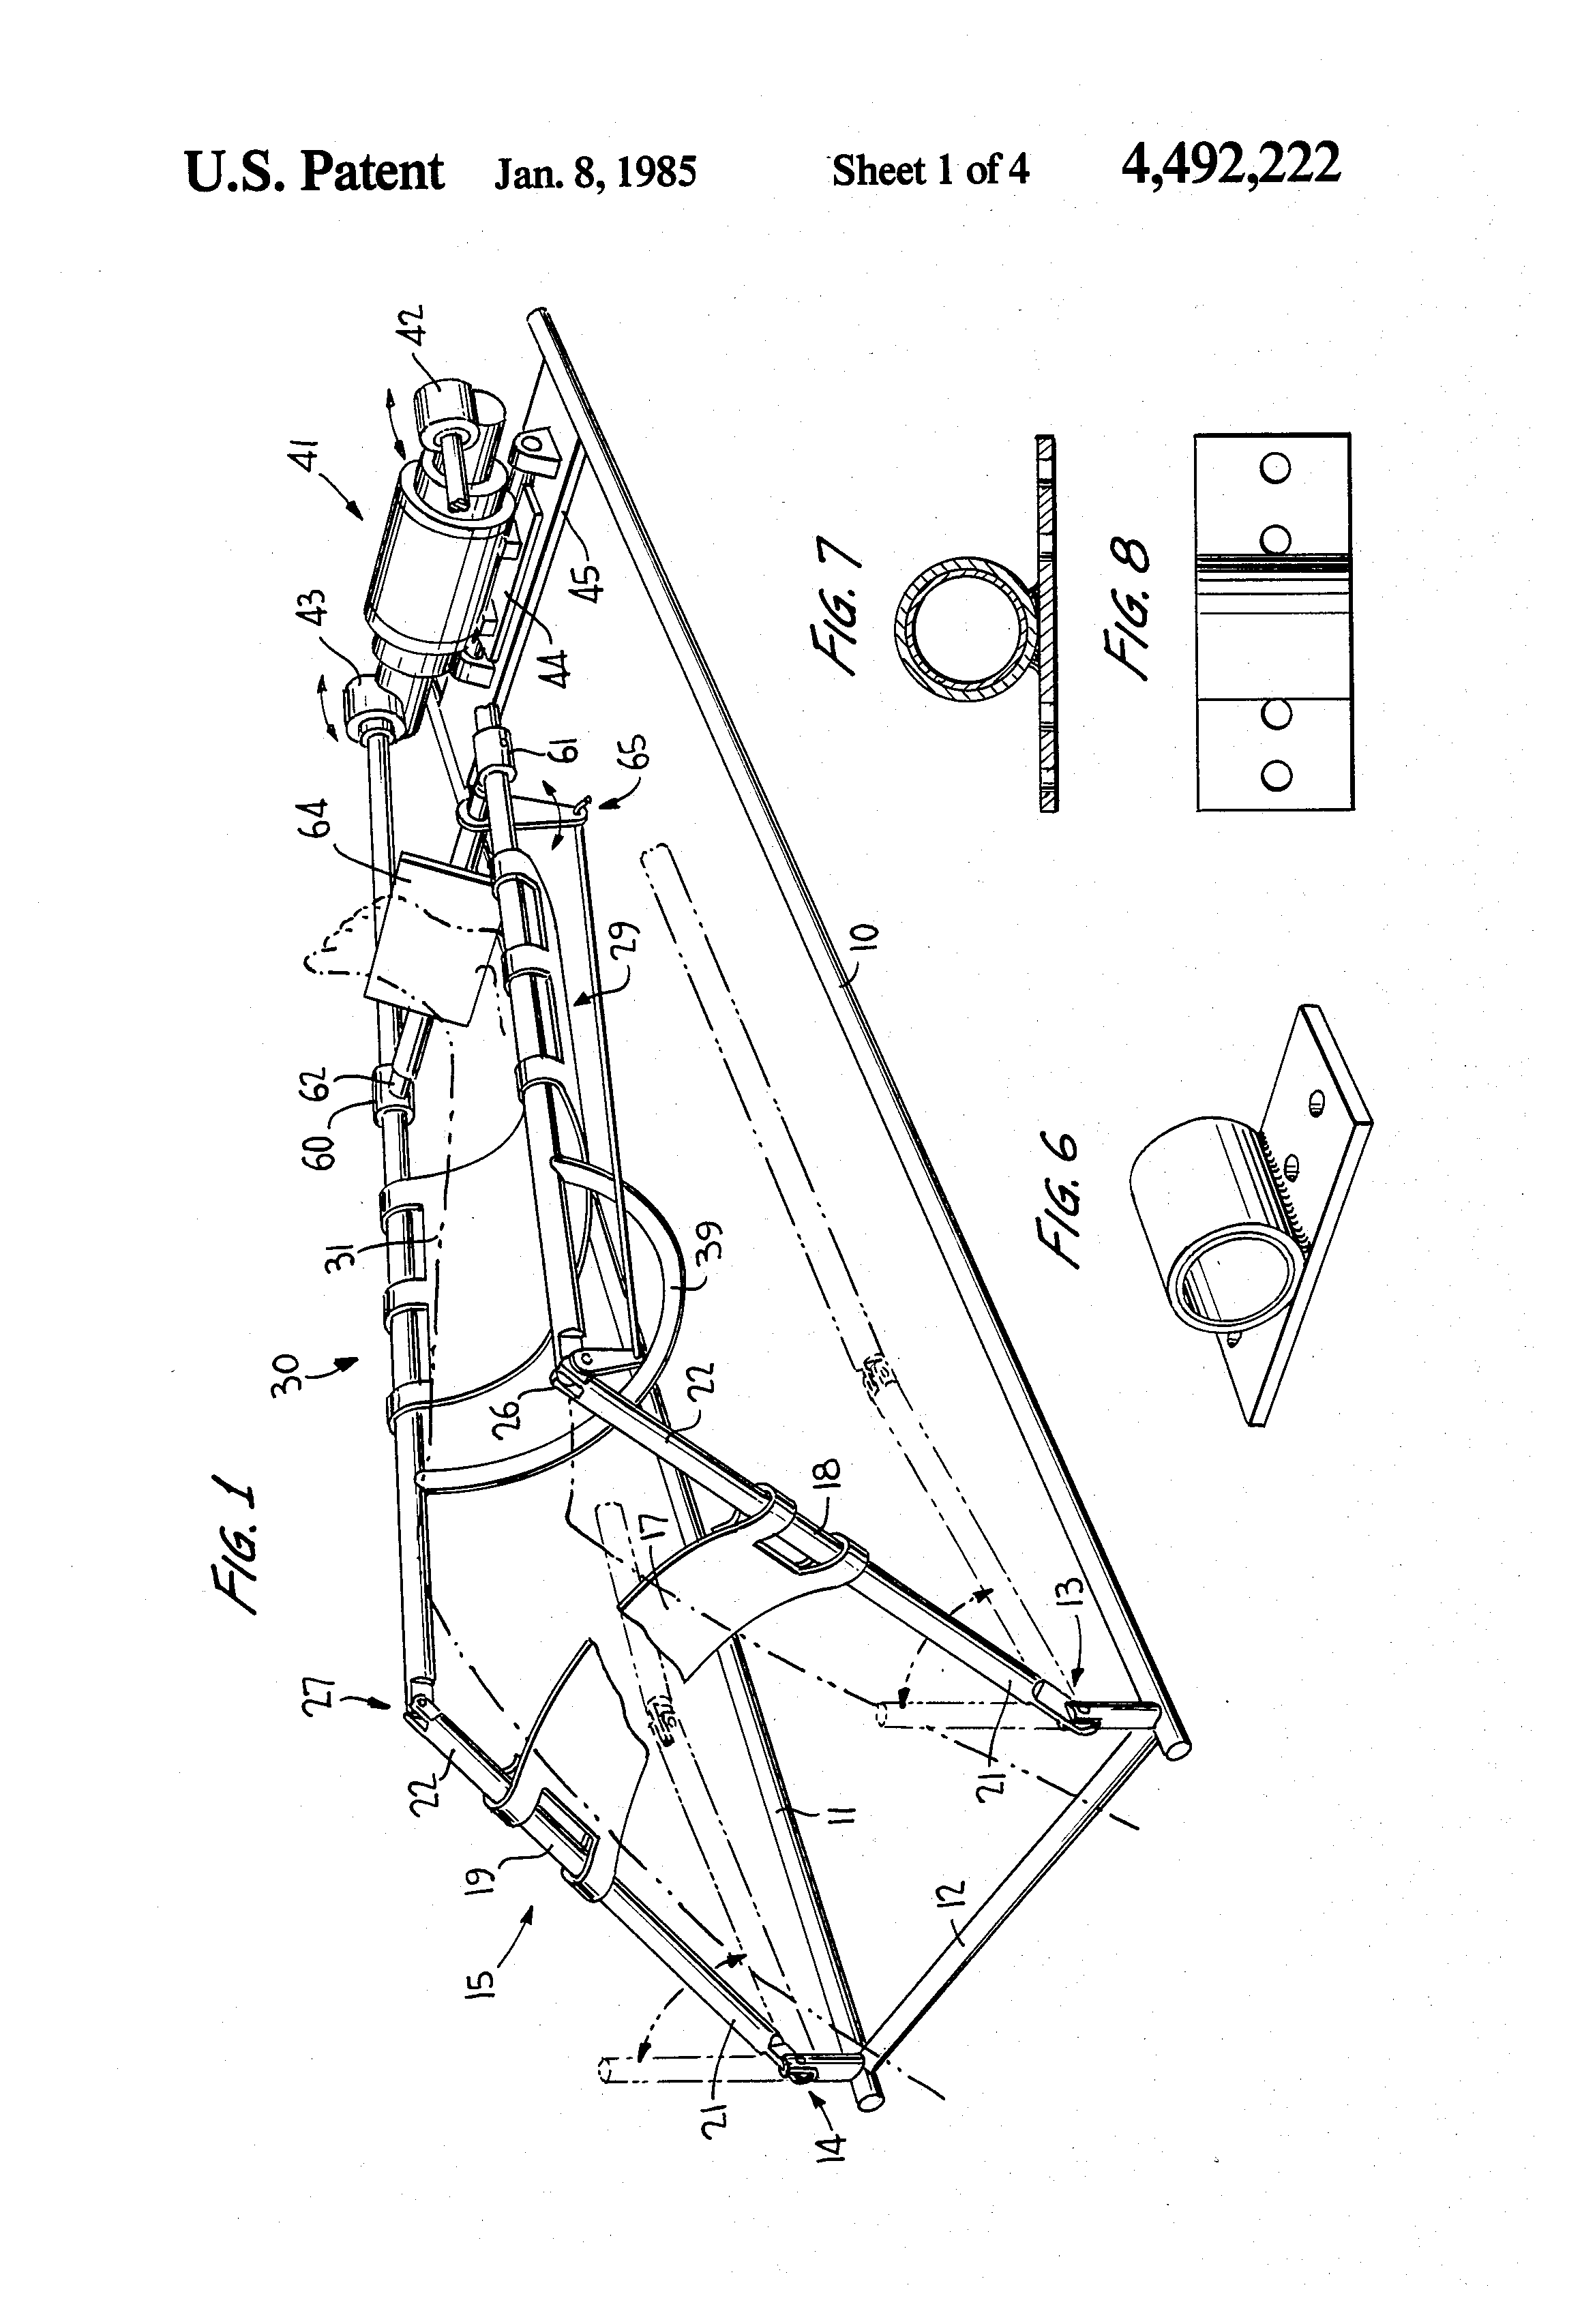
\includegraphics[width=0.54\linewidth]{4492222A_1.png}
  \caption{US4492222A knee exercise machine with adjustable axis alignment.}
  \label{fig:US4492222A}
\end{figure}

\subsection{Mechanism kinematics}

\section{US10272291B2: Knee Flexion and Extension Therapy Device and Method of Use}
\subsection{Description}
Modern therapy platform with modular brace interfaces and sensor-ready architecture for tracking compliance and motion. Highlights portability and user-centric controls to support clinic-to-home continuity.
\subsection{Images}
\begin{figure}[H]
  \centering
  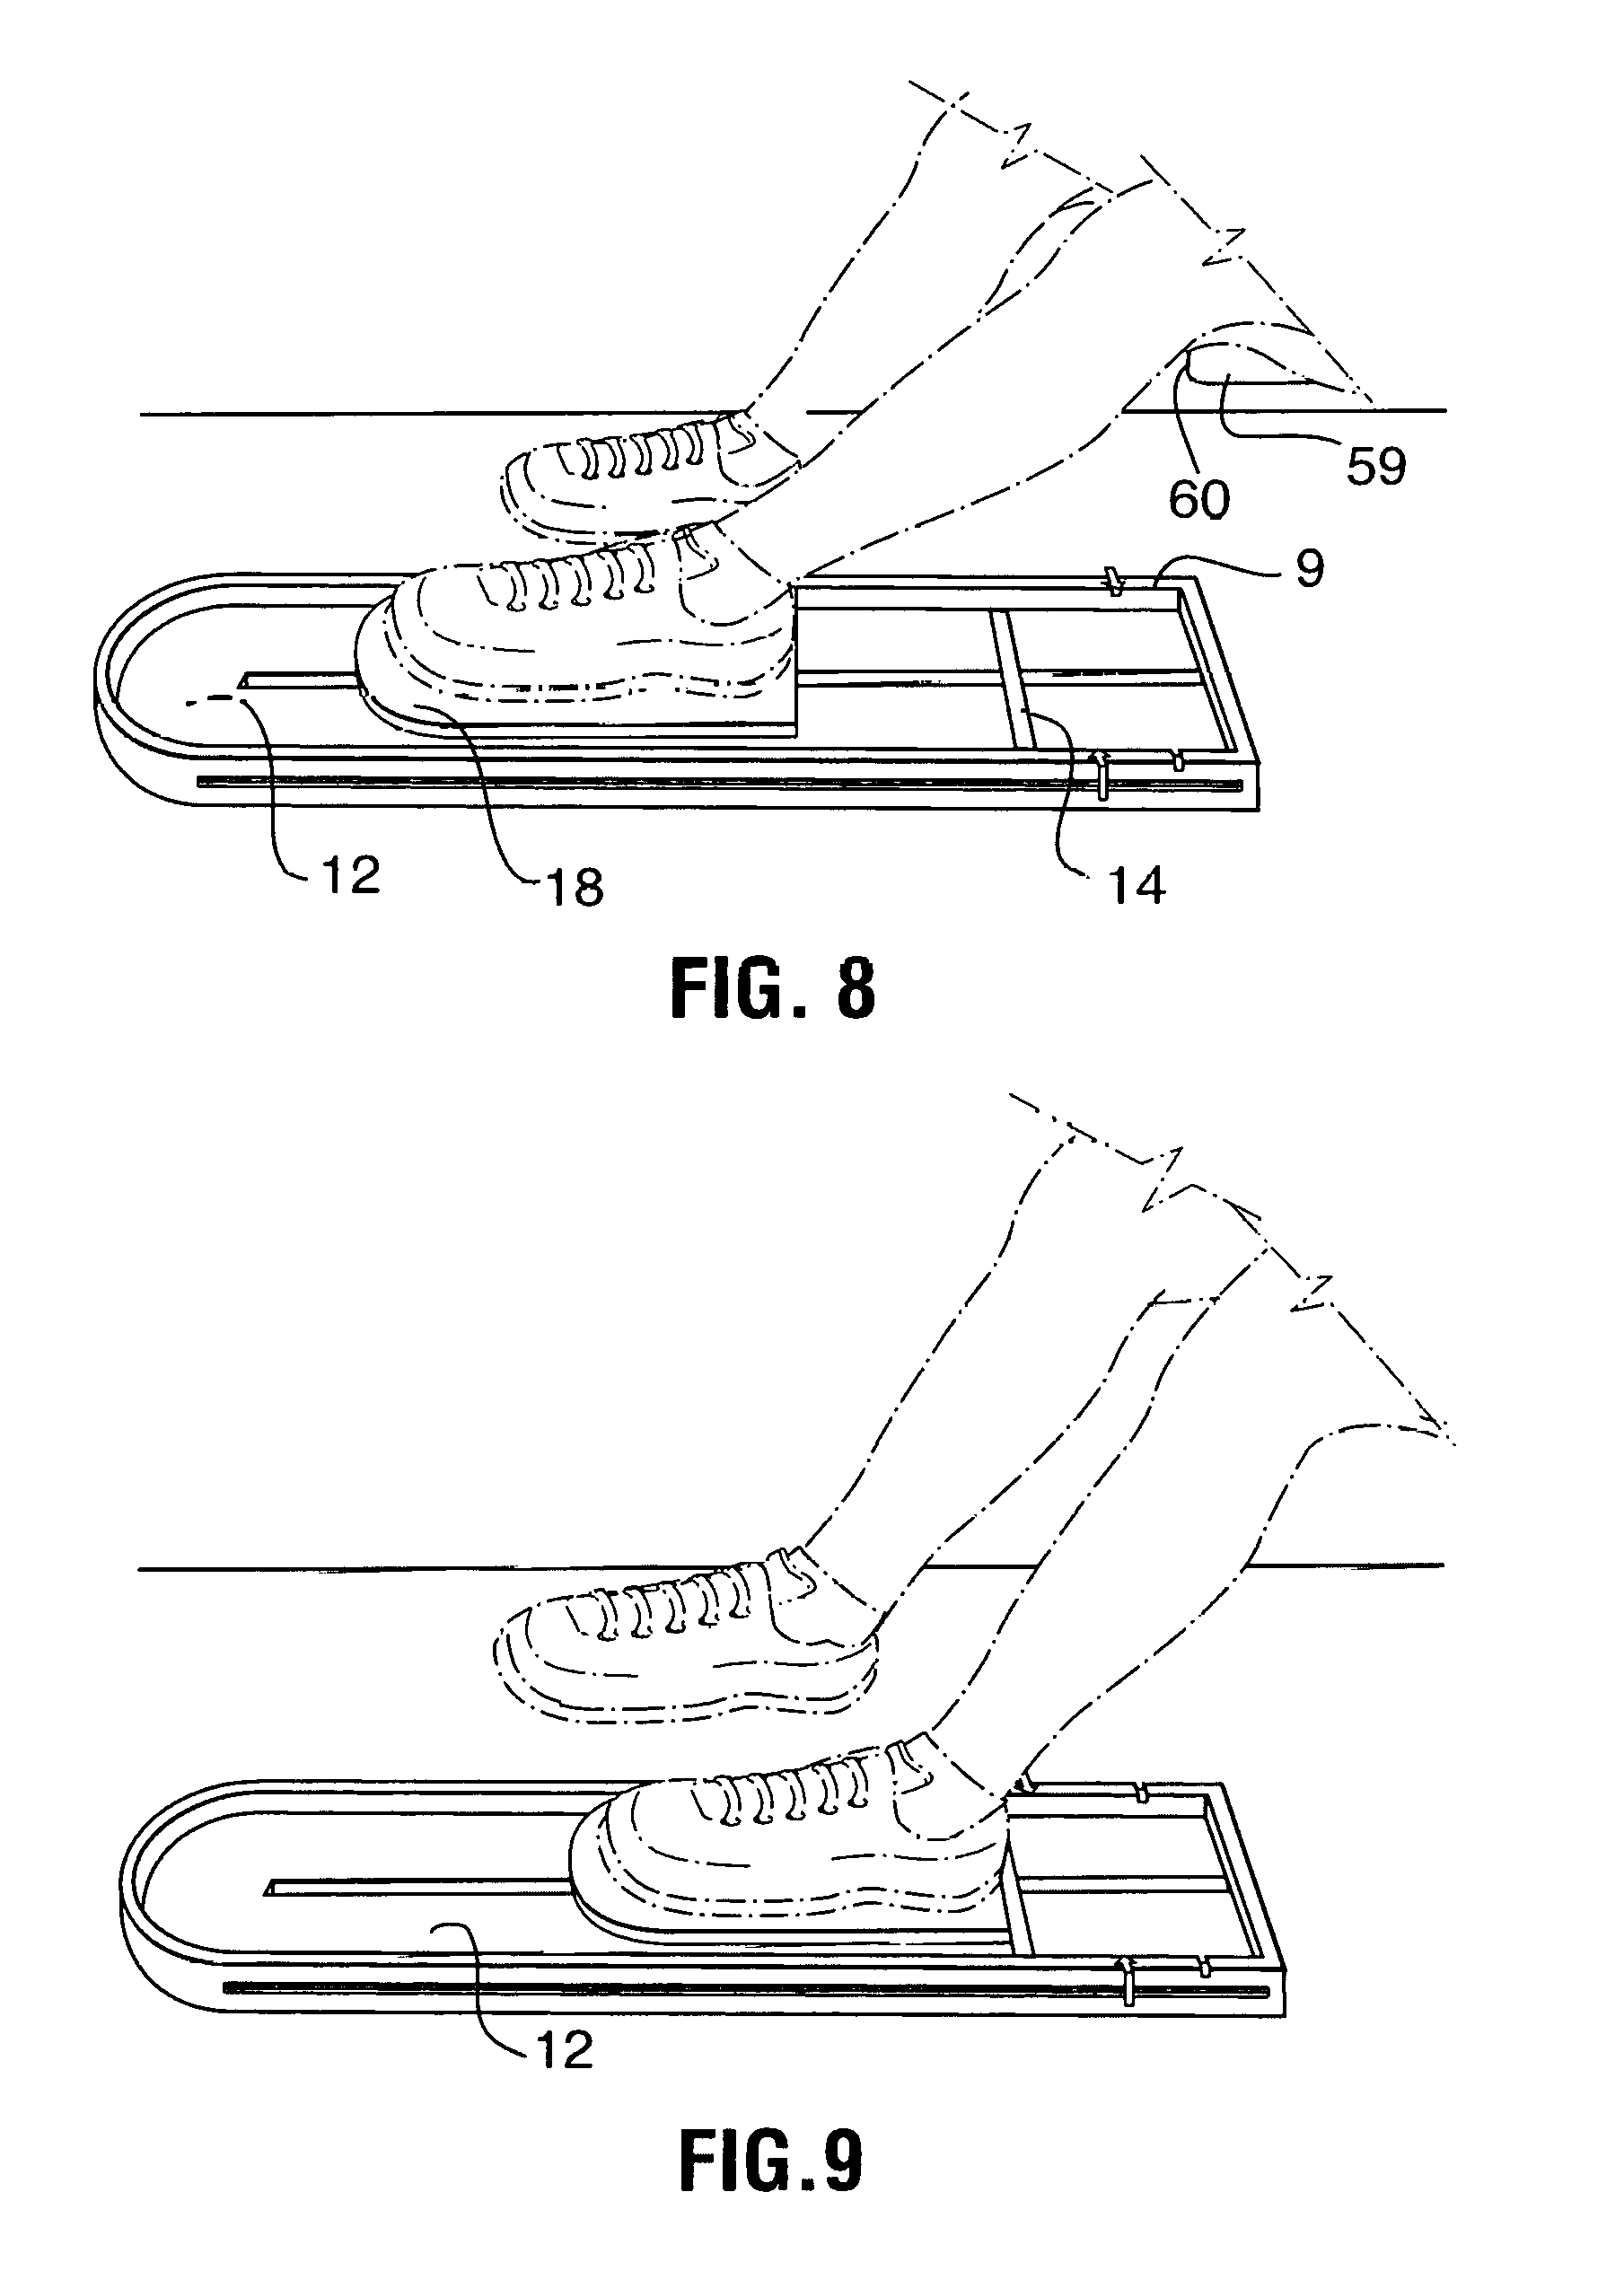
\includegraphics[width=0.54\linewidth]{10272291B2_1.png}
  \caption{US10272291B2 modern therapy platform for knee flexion/extension.}
  \label{fig:US10272291B2}
\end{figure}

\subsection{Mechanism kinematics}

\section{US4603687A: Continuous Passive Motion Orthopedic Device}
\subsection{Description}
Counterbalanced support arms with a motorized actuator and alignment aids to minimize off-axis loads. Designed for steady, repeatable cycles with straightforward mechanical adjustments.
\subsection{Images}
\begin{figure}[H]
  \centering
  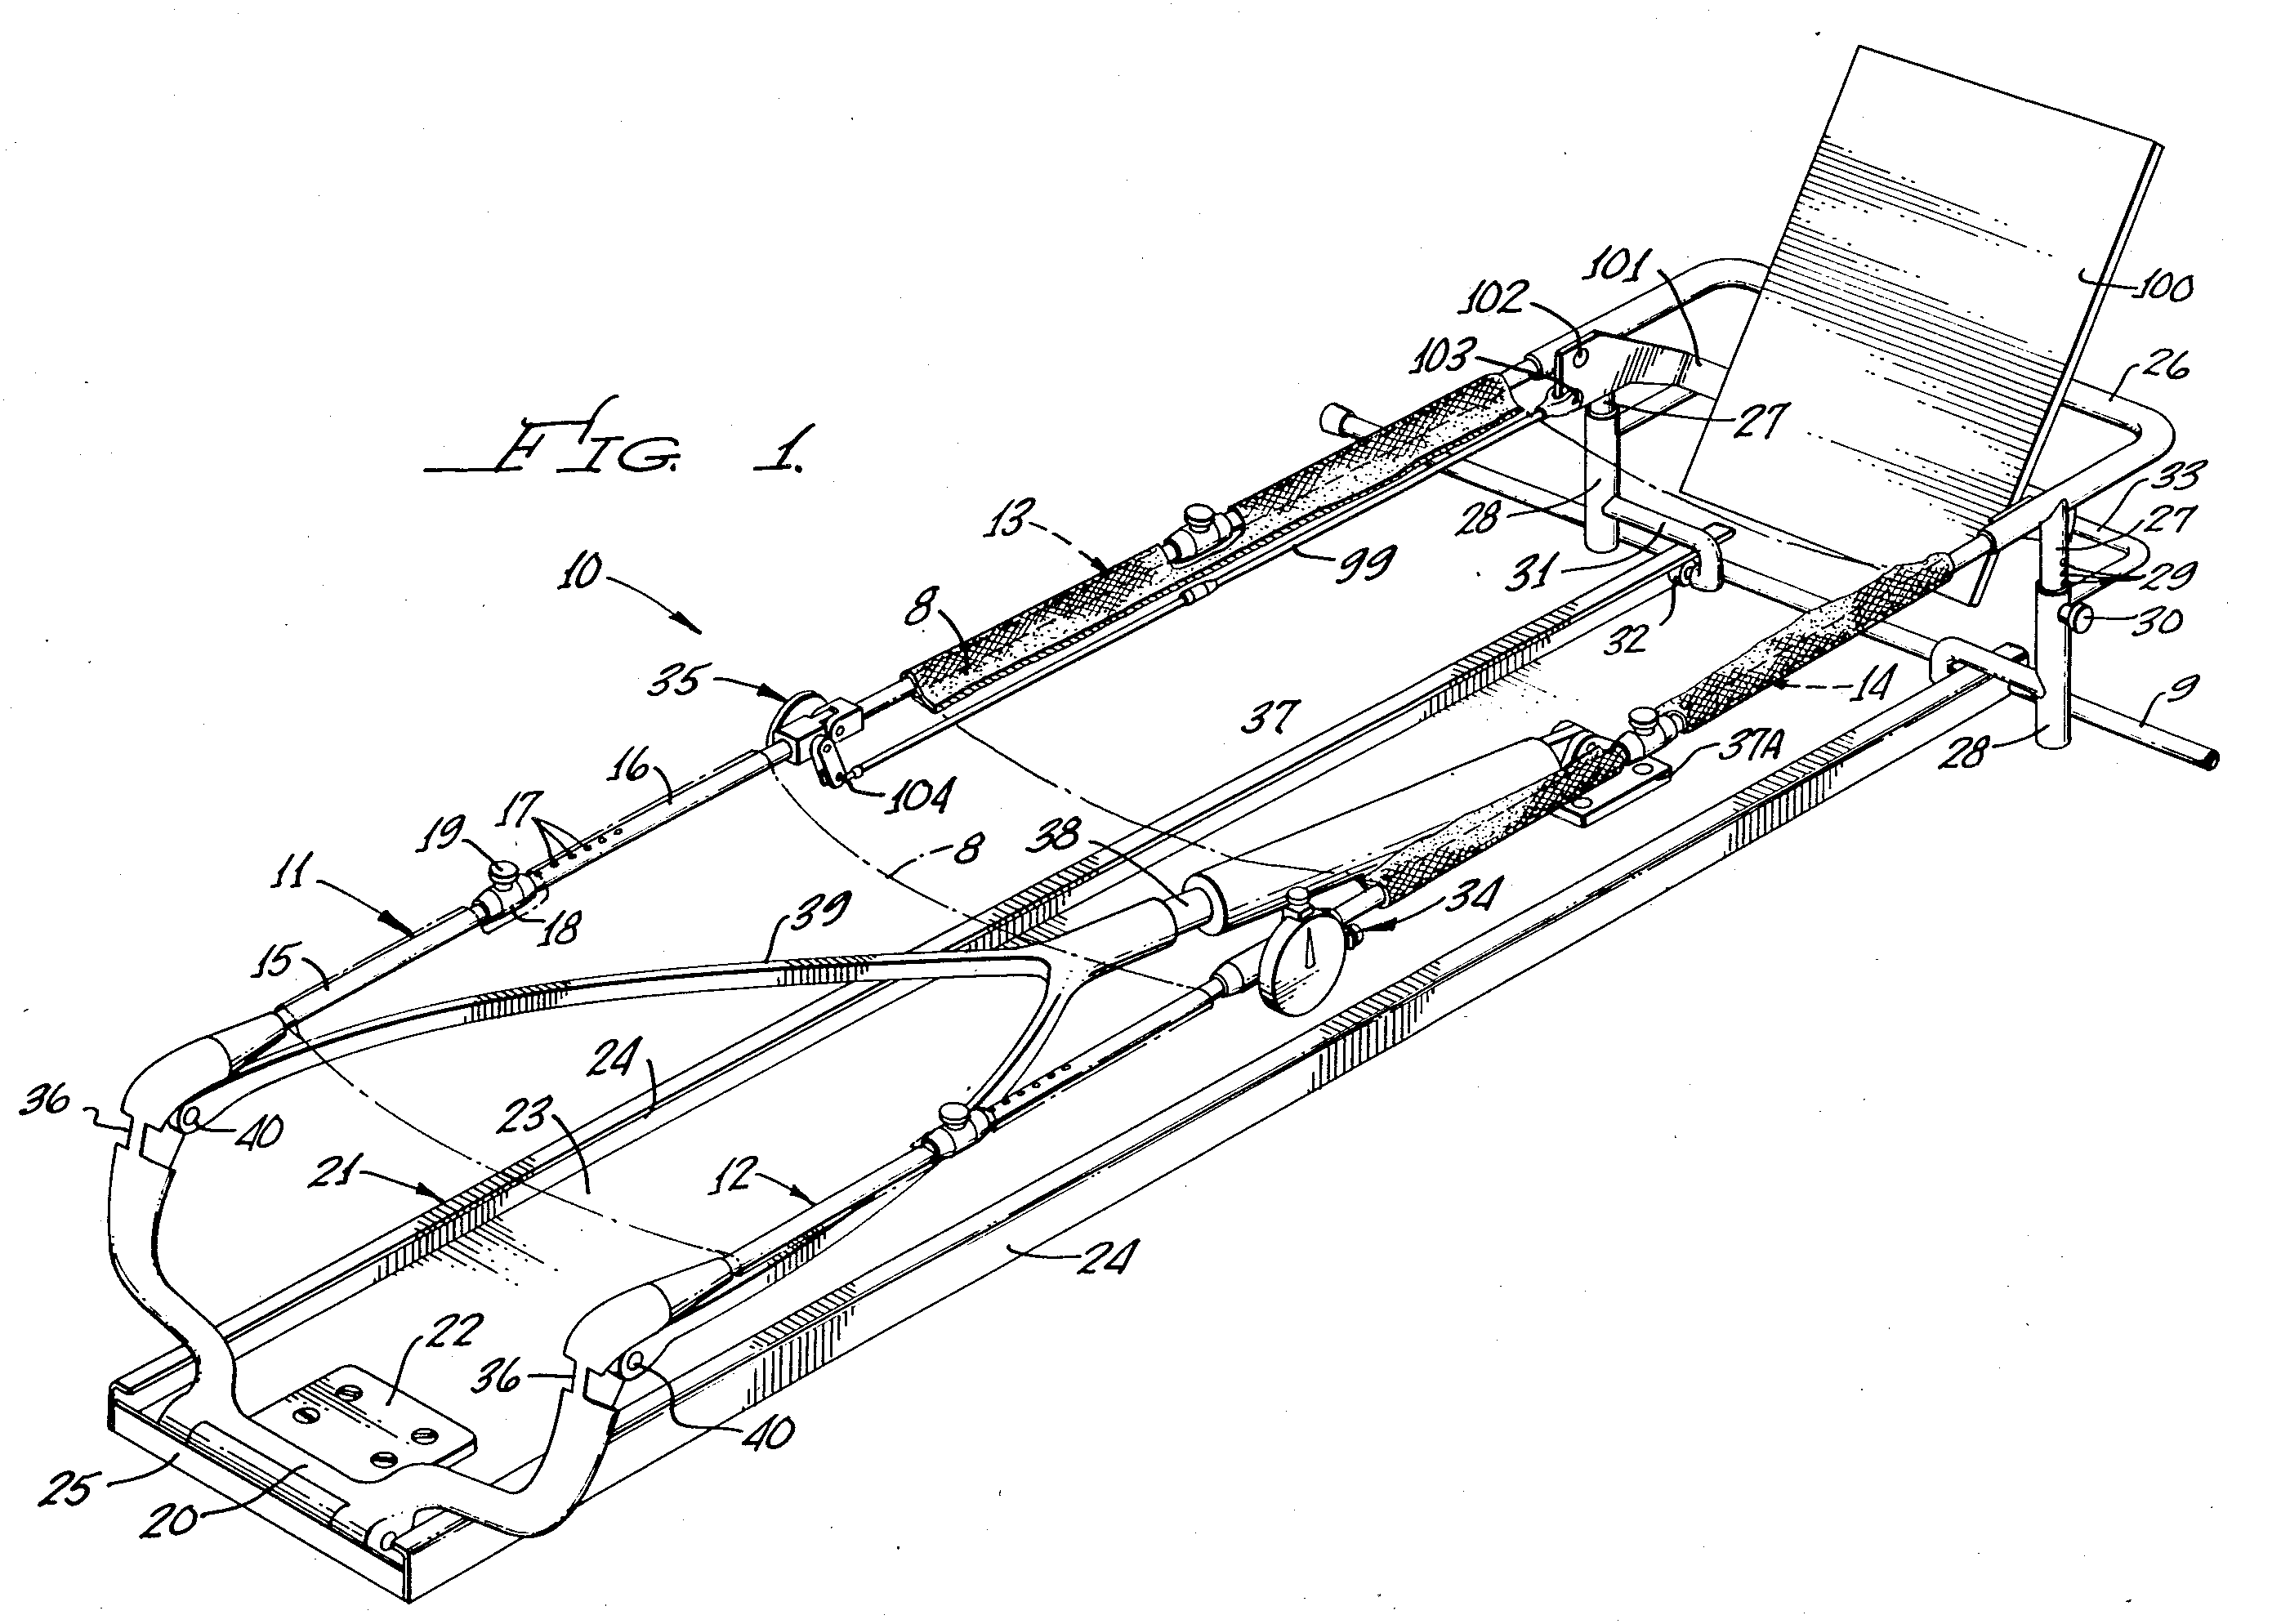
\includegraphics[width=0.54\linewidth]{US4603687_1.png}
  \caption{US4603687A CPM with counterbalanced arms and alignment aids.}
  \label{fig:US4603687A}
\end{figure}

\subsection{Mechanism kinematics}

\section{US5239987A: Anatomically Correct Continuous Passive Motion Device for a Limb}
\subsection{Description}
Axis-following mechanism intended to accommodate the knee’s migrating instantaneous center of rotation. Reduces misalignment-induced shear by adapting the motion path to a more anatomic \enquote{J-curve}.
\subsection{Images}
\begin{figure}[H]
  \centering
  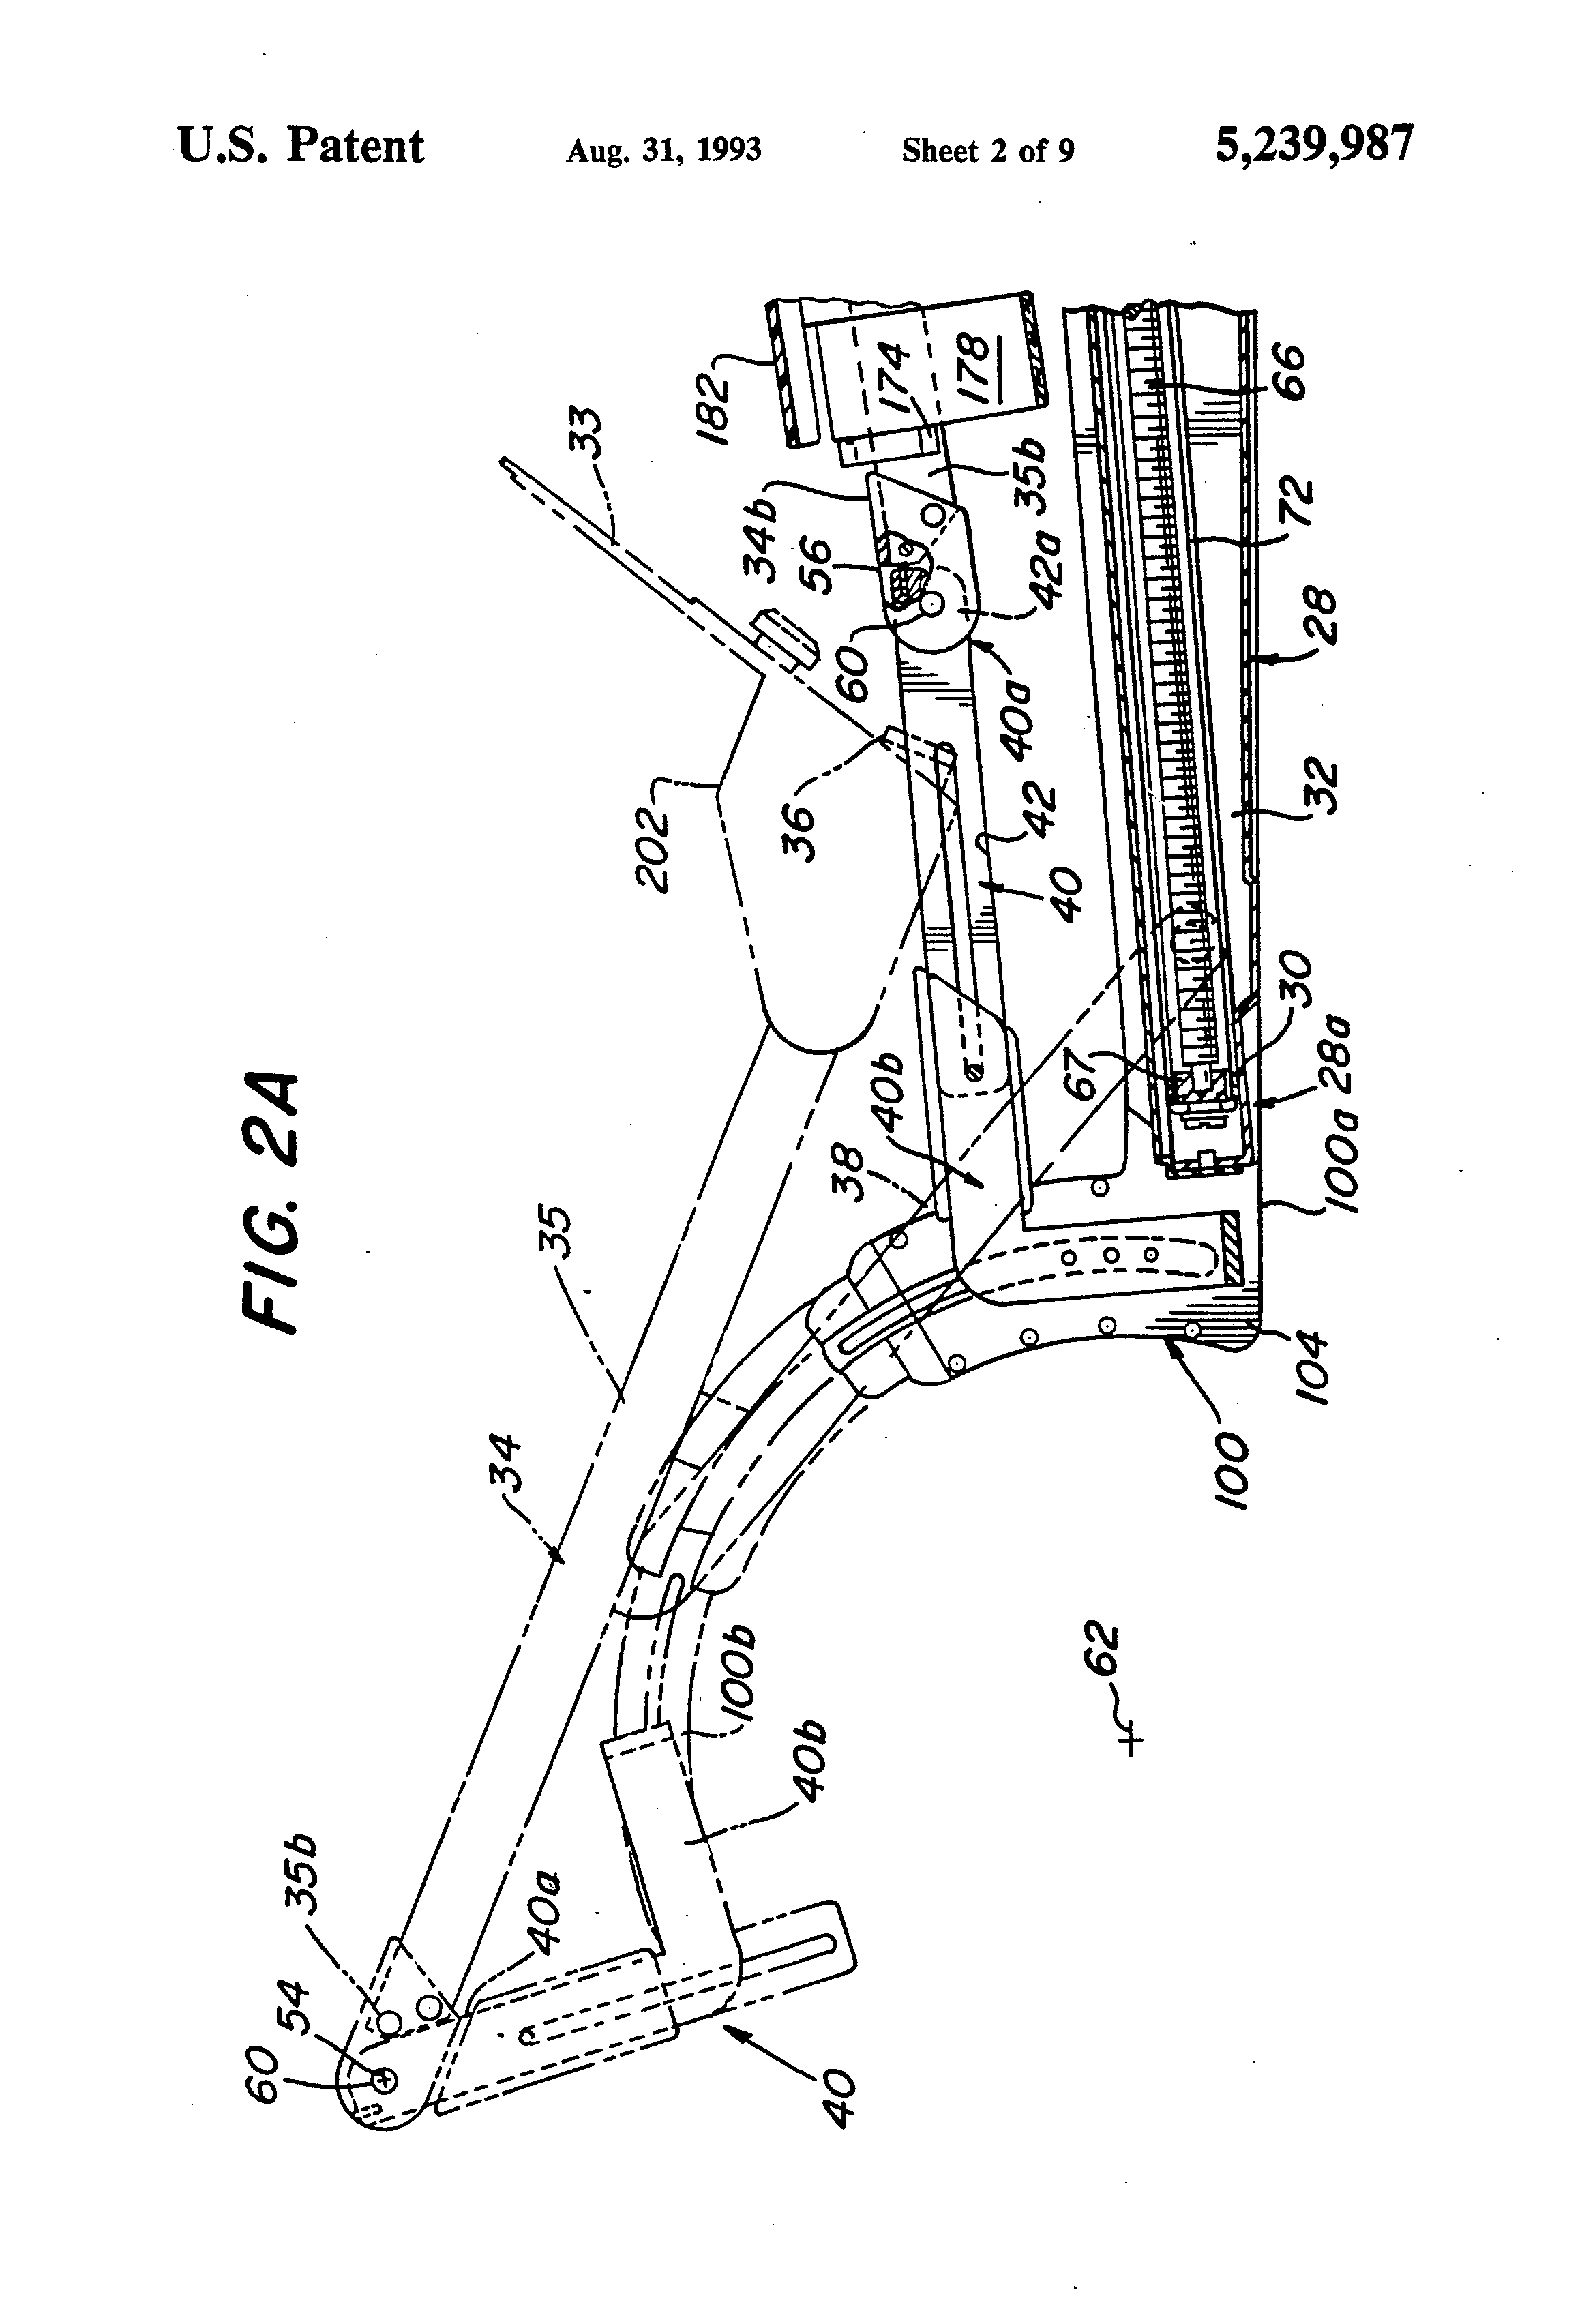
\includegraphics[width=0.54\linewidth]{US5239987-drawings-page-3.png}
  \caption{US5239987A device adapting to the knee’s shifting rotation center.}
  \label{fig:US5239987A}
\end{figure}

\subsection{Mechanism kinematics}

\section{US4546763A: Continuous Passive Motion Method and Apparatus}
\subsection{Description}
Claims both apparatus and therapy parameters, including programmable cycle timing, dwell at end range, and progressive ROM. Focuses on protocolization of CPM dosing alongside reliable mechanical delivery.
\subsection{Images}
\begin{figure}[H]
  \centering
  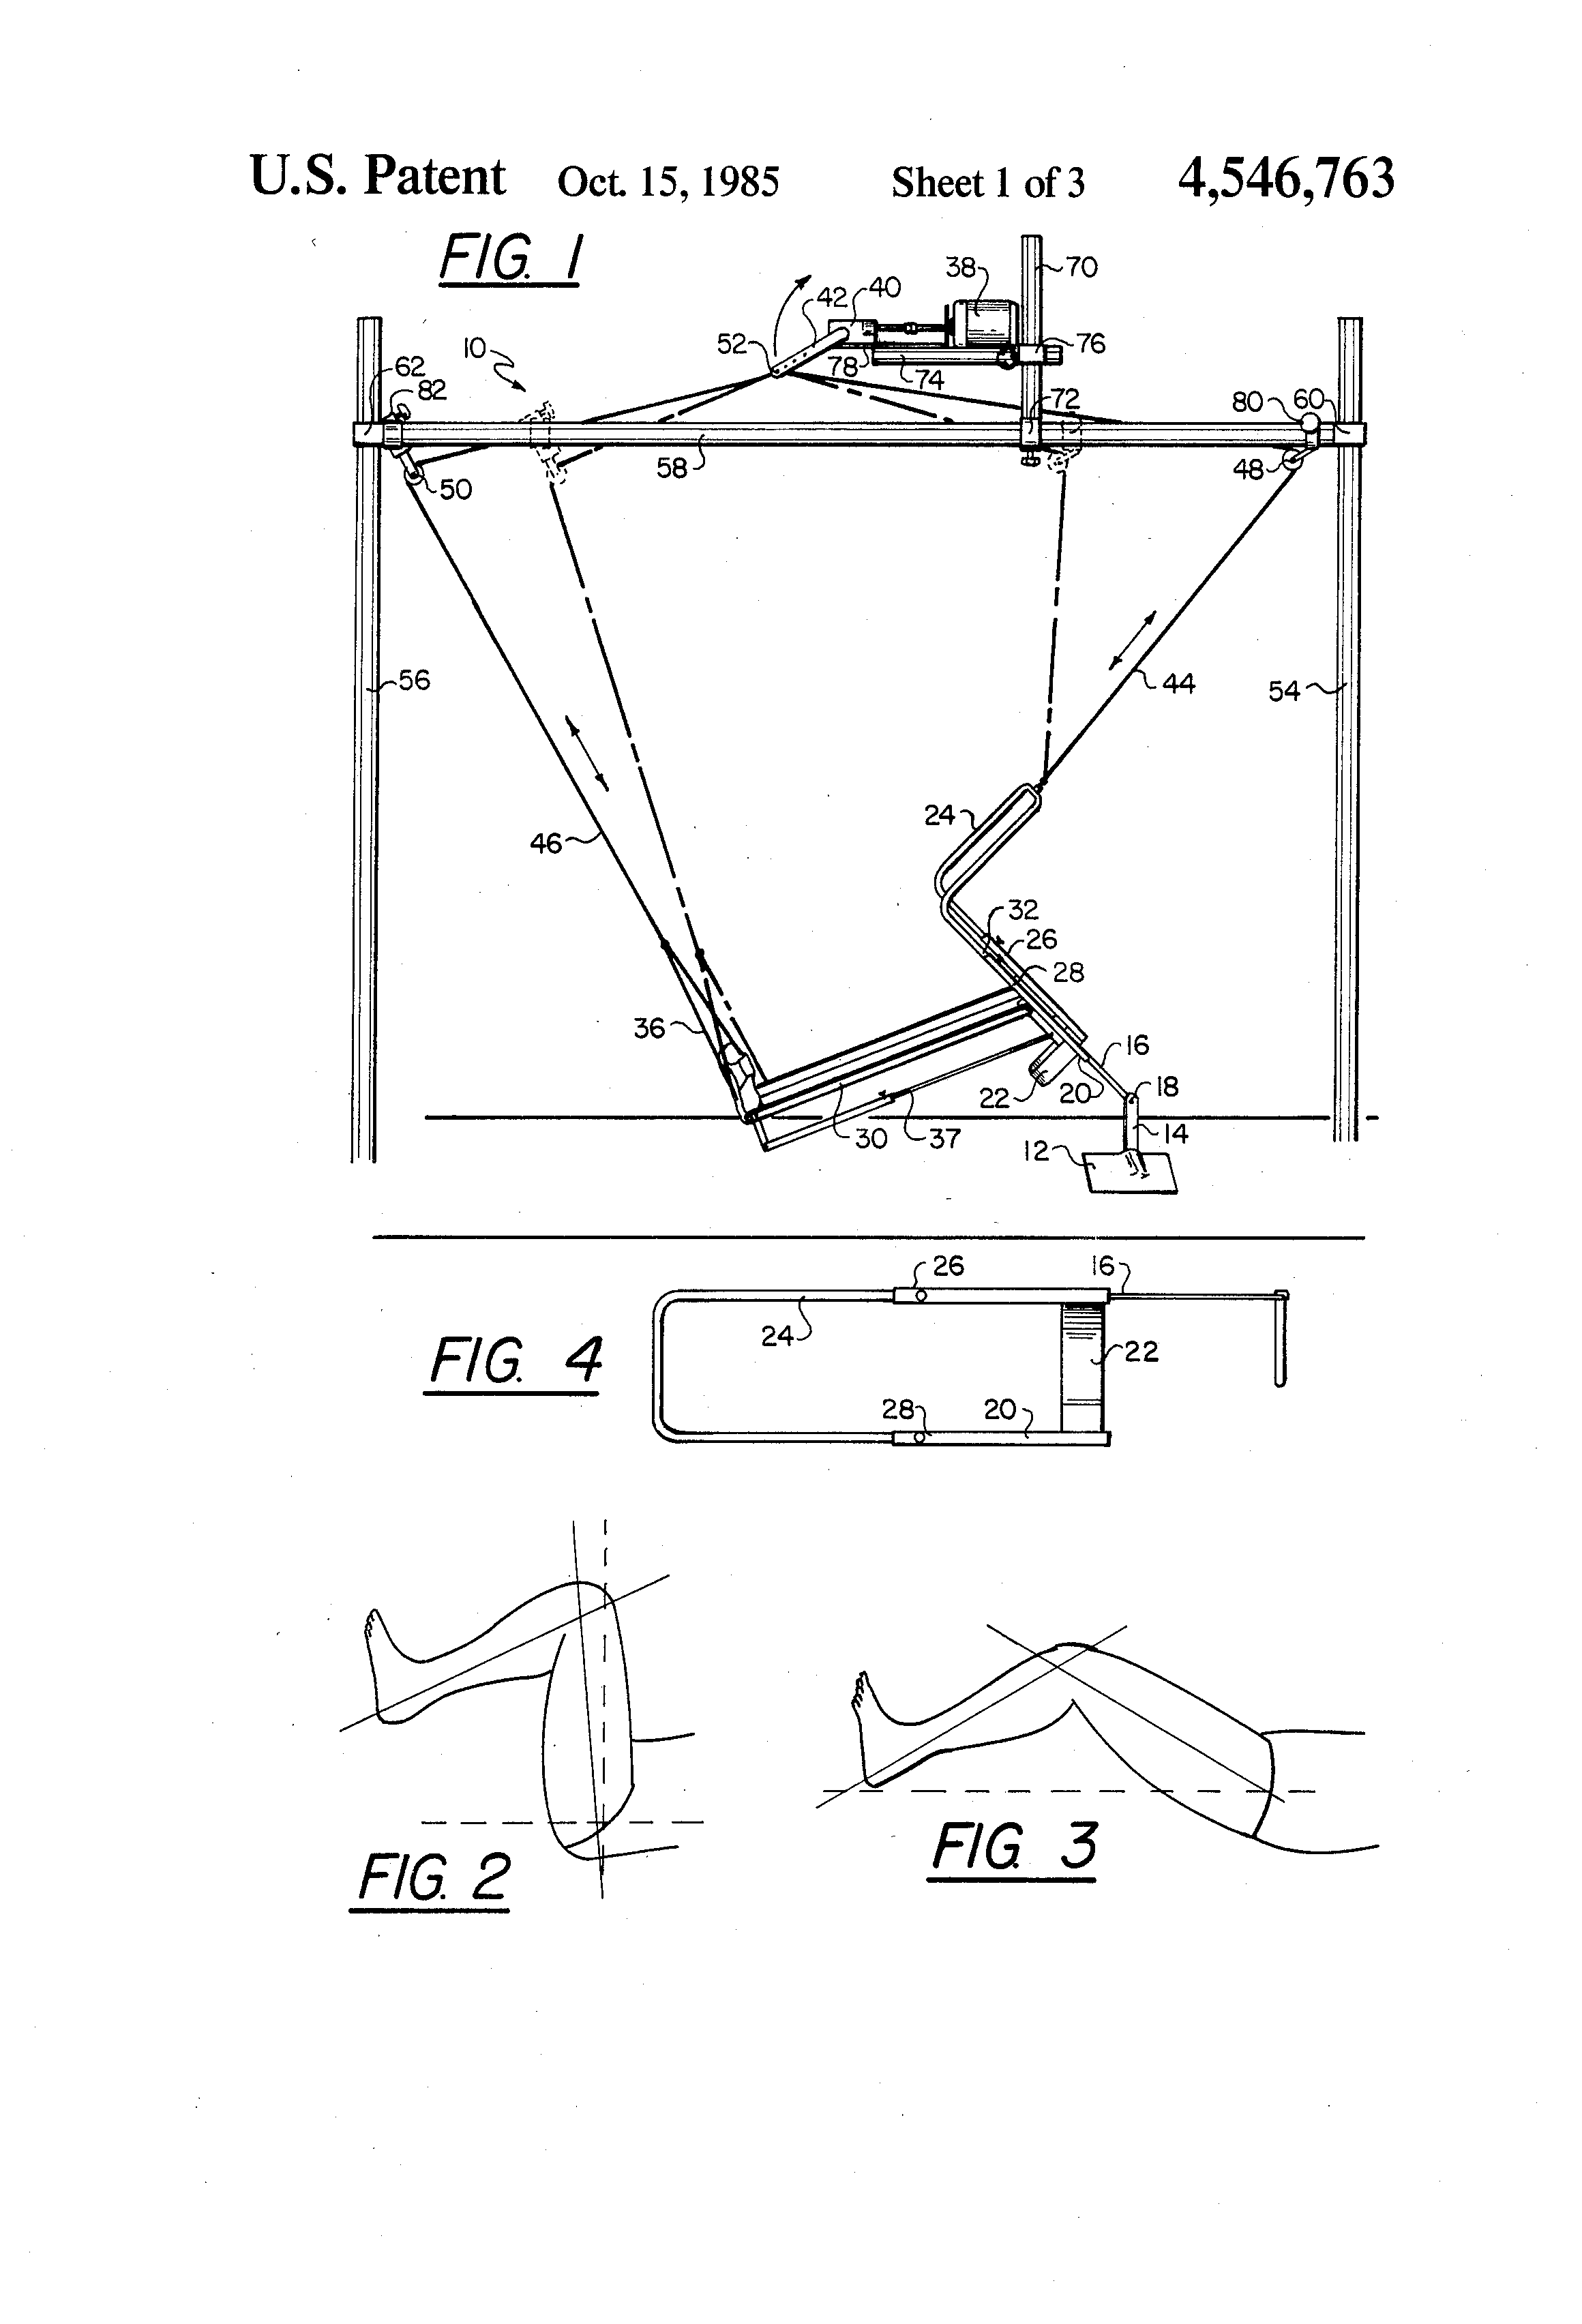
\includegraphics[width=0.54\linewidth]{US4546763-drawings-page-2.png}
  \caption{US4546763A apparatus and protocol emphasizing programmable CPM dosing.}
  \label{fig:US4546763A}
\end{figure}

\section{Methods}
Describe your approach, models, assumptions, and methodology in detail.

\section{Results}
Present results, figures, and tables. For example, include an image like in Figure~\ref{fig:example}.

\begin{figure}[h]
  \centering
  % \includegraphics[width=0.7\linewidth]{example.png}
  \caption{Example figure caption.}
  \label{fig:example}
\end{figure}

\section{Discussion}
Interpret the results, discuss limitations, and relate to prior work.

\section{Conclusion}
Summarize key takeaways and outline future work.

% If using BibTeX, uncomment the lines below and provide a references.bib file.
% \bibliographystyle{plain}
% \bibliography{references}

\end{document}


